%\RequirePackage{currfile}
\documentclass[12pt]{beamer}
\usepackage[utf8]{inputenc}
\usepackage[spanish]{babel}
\usepackage{standalone}
\usepackage{color}
\usepackage{siunitx}
\usepackage{hyperref}
%\hypersetup{colorlinks,linkcolor=,urlcolor=blue}
%\hypersetup{colorlinks,urlcolor=blue}
\usepackage{xcolor,soul}
\usepackage{etoolbox}
\usepackage{amsmath}
\usepackage{amsthm}
\usepackage{physics}
\usepackage{multicol}
\usepackage{bookmark}
\usepackage{longtable}
\usepackage{listings}
\usepackage{graphicx}
\usepackage{tikz}
\usetikzlibrary{patterns, matrix, backgrounds, decorations,shapes, arrows.meta}
\usepackage[autostyle,spanish=mexican]{csquotes}
\usepackage[os=win]{menukeys}
\usepackage{pifont}
\usepackage{pbox}
\usepackage{caption}
\captionsetup{font=scriptsize,labelfont=scriptsize}
%\usepackage[sfdefault]{roboto}  %% Option 'sfdefault' only if the base font of the document is to be sans serif

%Sección de definición de colores
\definecolor{ao}{rgb}{0.0, 0.5, 0.0}
\definecolor{bisque}{rgb}{1.0, 0.89, 0.77}
\definecolor{amber}{rgb}{1.0, 0.75, 0.0}
\definecolor{armygreen}{rgb}{0.29, 0.33, 0.13}
\definecolor{alizarin}{rgb}{0.82, 0.1, 0.26}
\definecolor{cadetblue}{rgb}{0.37, 0.62, 0.63}
\definecolor{deepblue}{rgb}{0,0,0.5}
\definecolor{brown}{rgb}{0.59, 0.29, 0.0}
\definecolor{OliveGreen}{rgb}{0,0.25,0}


\usefonttheme[onlymath]{serif}
%Sección de definición de nuevos comandos

\newcommand*{\TitleParbox}[1]{\parbox[c]{1.75cm}{\raggedright #1}}%
\newcommand{\python}{\texttt{python}}
\newcommand{\textoazul}[1]{\textcolor{blue}{#1}}
\newcommand{\azulfuerte}[1]{\textcolor{blue}{\textbf{#1}}}
\newcommand{\funcionazul}[1]{\textcolor{blue}{\textbf{\texttt{#1}}}}
\newcommand{\ptilde}[1]{\ensuremath{{#1}^{\prime}}}
\newcommand{\stilde}[1]{\ensuremath{{#1}^{\prime \prime}}}
\newcommand{\ttilde}[1]{\ensuremath{{#1}^{\prime \prime \prime}}}
\newcommand{\ntilde}[2]{\ensuremath{{#1}^{(#2)}}}
\renewcommand{\arraystretch}{1.5}

\newcounter{saveenumi}
\newcommand{\seti}{\setcounter{saveenumi}{\value{enumi}}}
\newcommand{\conti}{\setcounter{enumi}{\value{saveenumi}}}
\renewcommand{\rmdefault}{cmr}% cmr = Computer Modern Roman

\linespread{1.5}

\usefonttheme{professionalfonts}
%\usefonttheme{serif}
\DeclareGraphicsExtensions{.pdf,.png,.jpg}


%Sección para el tema de beamer, con el theme, usercolortheme y sección de footers
\mode<presentation>
{
  \usetheme{Madrid}
  \setbeamertemplate{headline}{}
  %\useoutertheme{infolines}
  \useoutertheme{default}
  \usecolortheme{beaver}
  \setbeamercovered{invisible}
  

  \setbeamertemplate{section in toc}[sections numbered]
  \setbeamertemplate{subsection in toc}[subsections numbered]
  \setbeamertemplate{subsection in toc}{\leavevmode\leftskip=3.2em\rlap{\hskip-2em\inserttocsectionnumber.\inserttocsubsectionnumber}\inserttocsubsection\par}
  \setbeamercolor{section in toc}{fg=blue}
  \setbeamercolor{subsection in toc}{fg=blue}
  \setbeamerfont{subsection in toc}{size=\small}
  \setbeamercolor{frametitle}{fg=blue}

  \setbeamertemplate{navigation symbols}{}
  \setbeamertemplate{caption}[numbered]

  %\beamertemplatenavigationsymbolsempty

  \makeatletter
  \setbeamercolor{section in foot}{bg=green!30!cyan, fg=black!90!orange}
  \setbeamercolor{subsection in foot}{bg=red!30!cyan, fg=red}
  %\setbeamercolor{date in foot}{bg=orange!30!cyan, fg=red}
  \setbeamertemplate{footline}
  {
    \leavevmode%
    \hbox{%
    \begin{beamercolorbox}[wd=.333333\paperwidth,ht=2.25ex,dp=1ex,center]{section in foot}%
      \usebeamerfont{section in foot} \insertsection
    \end{beamercolorbox}}%
    \begin{beamercolorbox}[wd=.333333\paperwidth,ht=2.25ex,dp=1ex,center]{subsection in foot}%
      \usebeamerfont{subsection in foot}  \insertsubsection
    \end{beamercolorbox}%
    \begin{beamercolorbox}[wd=.333333\paperwidth,ht=2.25ex,dp=1ex,right]{date in head/foot}%
      \usebeamerfont{date in head/foot} \insertshortdate{} \hspace*{2em}
      \insertframenumber{} / \inserttotalframenumber \hspace*{2ex} 
    \end{beamercolorbox}}%
    \vskip0pt%

  \makeatother

  \makeatletter
  \patchcmd{\beamer@sectionintoc}
    {\vfill}
    {\vskip\itemsep}
    {}
    {}
  \makeatother
  
}

% Sección para el código

\definecolor{Code}{rgb}{0,0,0}
\definecolor{Keywords}{rgb}{255,0,0}
\definecolor{Strings}{rgb}{255,0,255}
\definecolor{Comments}{rgb}{0,0,255}
\definecolor{Numbers}{rgb}{255,128,0}

\DeclareCaptionFont{white}{\color{white}}
\DeclareCaptionFormat{listing}{\colorbox{gray}{\parbox{0.99\textwidth}{#1#2#3}}}
\captionsetup[lstlisting]{format=listing,labelfont=white,textfont=white}
\renewcommand{\lstlistingname}{Código}

\lstset{
basicstyle=\ttfamily,
columns=fullflexible,
breaklines=true
}

\lstdefinestyle{codigopython}{%
  language=Python,                % choose the language of the code
  %basicstyle=\footnotesize\small,       % the size of the fonts that are used for the code
  numbers=left,                   % where to put the line-numbers
  numberstyle=\scriptsize,      % the size of the fonts that are used for the line-numbers
  stepnumber=1,                   % the step between two line-numbers. If it is 1 each line will be numbered
  numbersep=5pt,                  % how far the line-numbers are from the code
  backgroundcolor=\color{white},  % choose the background color. You must add \usepackage{color}
  showspaces=false,               % show spaces adding particular underscores
  showstringspaces=false,         % underline spaces within strings
  showtabs=false,                 % show tabs within strings adding particular underscores
  frame=single,   		% adds a frame around the code
  tabsize=2,  		% sets default tabsize to 2 spaces
  captionpos=t,   		% sets the caption-position to bottom
  breaklines=true,    	% sets automatic line breaking
  breakatwhitespace=false,    % sets if automatic breaks should only happen at whitespace
  escapeinside={\#},  % if you want to add a comment within your code
  stringstyle =\color{OliveGreen},
  texcl = true,
  %otherkeywords={{as}},             % Add keywords here
  keywordstyle = \color{blue},
  commentstyle = \color{black},
  identifierstyle = \color{black},
  % literate=%
  %         {á}{{\'a}}1
  %         {é}{{\'e}}1
  %         {í}{{\'i}}1
  %         {ó}{{\'o}}1
  %         {ú}{{\'u}}1
  %
  %keywordstyle=\ttb\color{deepblue}
  %fancyvrb = true,
literate={0}{{\textcolor{red}{0}}}{1}%
            {1}{{\textcolor{red}{1}}}{1}%
            {2}{{\textcolor{red}{2}}}{1}%
            {3}{{\textcolor{red}{3}}}{1}%
            {4}{{\textcolor{red}{4}}}{1}%
            {5}{{\textcolor{red}{5}}}{1}%
            {6}{{\textcolor{red}{6}}}{1}%
            {7}{{\textcolor{red}{7}}}{1}%
            {8}{{\textcolor{red}{8}}}{1}%
            {9}{{\textcolor{red}{9}}}{1}%
            {.0}{{\textcolor{red}{.0}}}{2}% Following is to ensure that only periods
            {.1}{{\textcolor{red}{.1}}}{2}% followed by a digit are changed.
            {.2}{{\textcolor{red}{.2}}}{2}%
            {.3}{{\textcolor{red}{.3}}}{2}%
            {.4}{{\textcolor{red}{.4}}}{2}%
            {.5}{{\textcolor{red}{.5}}}{2}%
            {.6}{{\textcolor{red}{.6}}}{2}%
            {.7}{{\textcolor{red}{.7}}}{2}%
            {.8}{{\textcolor{red}{.8}}}{2}%
            {.9}{{\textcolor{red}{.9}}}{2}%
            {\ }{{ }}{1}% handle the space
        ,%
        %mathescape=true
        %escapeinside={*@}
        escapeinside={A_}{_B}
}

%\RequirePackage[l2tabu, orthodox]{nag}
\RequirePackage{currfile}
\documentclass[12pt]{beamer}
\graphicspath{{Imagenes/}{../Imagenes/}}
\usepackage[utf8]{inputenc}
\usepackage[spanish]{babel}
\usepackage{standalone}
\usepackage{color}
\usepackage[binary-units=true]{siunitx}
\usepackage{hyperref}
\hypersetup{
  colorlinks=true,
  linkcolor=blue,          % color of internal links (change box color with linkbordercolor)
  citecolor=green,        % color of links to bibliography
  filecolor=magenta,      % color of file links
  urlcolor=cyan,           % color of external links
  linkbordercolor={0 0 1}
}
\usepackage{xcolor, soul}
\usepackage{etoolbox}
\usepackage{amsmath}
\usepackage{amsthm}
\usepackage{physics}
\usepackage{multicol}
\usepackage{graphicx}
\usepackage{bookmark}
\usepackage{longtable}
\usepackage{graphicx}
\usepackage{tikz}
\usepackage[siunitx, RPvoltages]{circuitikz}
\usetikzlibrary{mindmap}
\usetikzlibrary{arrows, patterns, shapes, decorations.markings, decorations.pathmorphing}
\usetikzlibrary{matrix,positioning}
\tikzstyle{every picture}+=[remember picture,baseline]
\usepackage[autostyle,spanish=mexican]{csquotes}
\usepackage{pifont}
\usepackage[font=footnotesize,textfont=it]{caption}
\usepackage{tabulary}
\usepackage{booktabs}
\usepackage[outdir=./]{epstopdf}
%\usepackage{epstopdf}
\usepackage{media9}
\usepackage{multimedia}
\usepackage{bigints}
%\usepackage{enumitem}
\usepackage[os=win]{menukeys}
\usepackage{pifont}
\usepackage{pbox}
\usepackage{alltt}
\usepackage{verbatim}
\usepackage{colortbl}
\usepackage{tcolorbox}
\usepackage{fancyvrb}
\usepackage[sfdefault]{roboto}  %% Option 'sfdefault' only if the base font of the document is to be sans serif
%\usepackage[T1]{fontenc}
\setcounter{secnumdepth}{3}
\setcounter{tocdepth}{3}
\DeclareGraphicsExtensions{.pdf,.png,.jpg}
\renewcommand {\arraystretch}{1.5}
\definecolor{ao}{rgb}{0.0, 0.5, 0.0}
\definecolor{aquamarine}{rgb}{0.5, 1.0, 0.83}
\definecolor{kellygreen}{rgb}{0.3, 0.73, 0.09}
\definecolor{bisque}{rgb}{1.0, 0.89, 0.77}
\definecolor{amber}{rgb}{1.0, 0.75, 0.0}
\definecolor{armygreen}{rgb}{0.29, 0.33, 0.13}
\definecolor{alizarin}{rgb}{0.82, 0.1, 0.26}
\definecolor{cadetblue}{rgb}{0.37, 0.62, 0.63}
\newcommand*{\TitleParbox}[1]{\parbox[c]{6cm}{\raggedright #1}}%
\newcommand{\python}{\texttt{python}}
\newcommand{\textoazul}[1]{\textcolor{blue}{#1}}
\newcommand{\azulfuerte}[1]{\textcolor{blue}{\textbf{#1}}}
\newcommand{\funcionazul}[1]{\textcolor{blue}{\textbf{\texttt{#1}}}}
%\normalfont
\usepackage{ccfonts}% http://ctan.org/pkg/{ccfonts}
\usepackage[T1]{fontenc}% http://ctan.or/pkg/fontenc
\renewcommand{\rmdefault}{cmr}% cmr = Computer Modern Roman
\usefonttheme[onlymath]{serif}
\linespread{1.3}
\newcounter{saveenumi}
\newcommand{\seti}{\setcounter{saveenumi}{\value{enumi}}}
\newcommand{\conti}{\setcounter{enumi}{\value{saveenumi}}}
\newcommand{\tikzmark}[1]{\tikz[remember picture] \node[coordinate] (#1) {#1};}

\usepackage{scalerel}[2016-12-29]
\def\stretchint#1{\vcenter{\hbox{\stretchto[440]{\displaystyle\int}{#1}}}}
\def\scaleint#1{\vcenter{\hbox{\scaleto[3ex]{\displaystyle\int}{#1}}}}
\def\bs{\mkern-12mu}

\newtheorem{teo}{}[section]
\usepackage{blkarray}

%reduce el tamaño de letra de la etiqueta equations
\makeatletter
\def\maketag@@@#1{\hbox{\m@th\normalfont\small#1}}
\makeatother

%se usa para la x en itemize
\newcommand{\xmark}{\text{\ding{55}}}

%\AtBeginDocument{\setlength{\tymin}{1em}}


\definecolor{myblue}{rgb}{.8, .8, 1}

\usepackage{empheq}

\newlength\mytemplen
\newsavebox\mytempbox

\makeatletter
\newcommand\mybluebox{%
    \@ifnextchar[%]
       {\@mybluebox}%
       {\@mybluebox[0pt]}}

\def\@mybluebox[#1]{%
    \@ifnextchar[%]
       {\@@mybluebox[#1]}%
       {\@@mybluebox[#1][0pt]}}

\def\@@mybluebox[#1][#2]#3{
    \sbox\mytempbox{#3}%
    \mytemplen\ht\mytempbox
    \advance\mytemplen #1\relax
    \ht\mytempbox\mytemplen
    \mytemplen\dp\mytempbox
    \advance\mytemplen #2\relax
    \dp\mytempbox\mytemplen
    \colorbox{myblue}{\hspace{1em}\usebox{\mytempbox}\hspace{1em}}}

\makeatother



%Se usa la plantilla Madrid modificada con beaver
\mode<presentation>
{
  \usetheme{Madrid}
  \setbeamertemplate{headline}{}
  %\useoutertheme{infolines}
  \usecolortheme{beaver}
  \setbeamercovered{invisible}
  

\setbeamertemplate{section in toc}[sections numbered]
\setbeamertemplate{subsection in toc}[subsections numbered]
\setbeamertemplate{subsection in toc}{\leavevmode\leftskip=3.2em\rlap{\hskip-2em\inserttocsectionnumber.\inserttocsubsectionnumber}\inserttocsubsection\par}
\setbeamercolor{section in toc}{fg=blue}
\setbeamercolor{subsection in toc}{fg=blue}
\setbeamerfont{subsection in toc}{size=\small}

\setbeamertemplate{navigation symbols}{}
\setbeamertemplate{caption}[numbered]

}

\usepackage{courier}
\usepackage{listingsutf8}
\usepackage{listings}
\usepackage{xcolor}
\usepackage{textcomp}
\usepackage{color}
\definecolor{deepblue}{rgb}{0,0,0.5}
\definecolor{brown}{rgb}{0.59, 0.29, 0.0}
\definecolor{OliveGreen}{rgb}{0,0.25,0}
% \usepackage{minted}

\DeclareCaptionFont{white}{\color{white}}
\DeclareCaptionFormat{listing}{\colorbox{gray}{\parbox{0.98\textwidth}{#1#2#3}}}
\captionsetup[lstlisting]{format=listing,labelfont=white,textfont=white}
\renewcommand{\lstlistingname}{Código}


\definecolor{Code}{rgb}{0,0,0}
\definecolor{Keywords}{rgb}{255,0,0}
\definecolor{Strings}{rgb}{255,0,255}
\definecolor{Comments}{rgb}{0,0,255}
\definecolor{Numbers}{rgb}{255,128,0}

\makeatletter

\newif\iffirstchar\firstchartrue
\newif\ifstartedbyadigit
\newif\ifprecededbyequalsign

\newcommand\processletter
{%
  \ifnum\lst@mode=\lst@Pmode%
    \iffirstchar%
        \global\startedbyadigitfalse%
      \fi
      \global\firstcharfalse%
    \fi
}

\newcommand\processdigit
{%
  \ifnum\lst@mode=\lst@Pmode%
      \iffirstchar%
        \global\startedbyadigittrue%
      \fi
      \global\firstcharfalse%
  \fi
}

\lst@AddToHook{OutputOther}%
{%
  \lst@IfLastOtherOneOf{=}
    {\global\precededbyequalsigntrue}
    {}%
}

\lst@AddToHook{Output}%
{%
  \ifprecededbyequalsign%
      \ifstartedbyadigit%
        \def\lst@thestyle{\color{orange}}%
      \fi
    \fi
  \global\firstchartrue%
  \global\startedbyadigitfalse%
  \global\precededbyequalsignfalse%
}

\lstset{ 
language=Python,                % choose the language of the code
basicstyle=\footnotesize\ttfamily,       % the size of the fonts that are used for the code
numbers=left,                   % where to put the line-numbers
numberstyle=\scriptsize,      % the size of the fonts that are used for the line-numbers
stepnumber=1,                   % the step between two line-numbers. If it is 1 each line will be numbered
numbersep=5pt,                  % how far the line-numbers are from the code
backgroundcolor=\color{white},  % choose the background color. You must add \usepackage{color}
showspaces=false,               % show spaces adding particular underscores
showstringspaces=false,         % underline spaces within strings
showtabs=false,                 % show tabs within strings adding particular underscores
frame=single,   		% adds a frame around the code
tabsize=2,  		% sets default tabsize to 2 spaces
captionpos=t,   		% sets the caption-position to bottom
breaklines=true,    	% sets automatic line breaking
breakatwhitespace=false,    % sets if automatic breaks should only happen at whitespace
escapeinside={\#},  % if you want to add a comment within your code
stringstyle =\color{OliveGreen},
%otherkeywords={{as}},             % Add keywords here
keywordstyle = \color{blue},
commentstyle = \color{black},
identifierstyle = \color{black},
literate=%
         {á}{{\'a}}1
         {é}{{\'e}}1
         {í}{{\'i}}1
         {ó}{{\'o}}1
         {ú}{{\'u}}1
%
%keywordstyle=\ttb\color{deepblue}
%fancyvrb = true,
}

\lstdefinestyle{FormattedNumber}{%
    literate={0}{{\textcolor{red}{0}}}{1}%
             {1}{{\textcolor{red}{1}}}{1}%
             {2}{{\textcolor{red}{2}}}{1}%
             {3}{{\textcolor{red}{3}}}{1}%
             {4}{{\textcolor{red}{4}}}{1}%
             {5}{{\textcolor{red}{5}}}{1}%
             {6}{{\textcolor{red}{6}}}{1}%
             {7}{{\textcolor{red}{7}}}{1}%
             {8}{{\textcolor{red}{8}}}{1}%
             {9}{{\textcolor{red}{9}}}{1}%
             {.0}{{\textcolor{red}{.0}}}{2}% Following is to ensure that only periods
             {.1}{{\textcolor{red}{.1}}}{2}% followed by a digit are changed.
             {.2}{{\textcolor{red}{.2}}}{2}%
             {.3}{{\textcolor{red}{.3}}}{2}%
             {.4}{{\textcolor{red}{.4}}}{2}%
             {.5}{{\textcolor{red}{.5}}}{2}%
             {.6}{{\textcolor{red}{.6}}}{2}%
             {.7}{{\textcolor{red}{.7}}}{2}%
             {.8}{{\textcolor{red}{.8}}}{2}%
             {.9}{{\textcolor{red}{.9}}}{2}%
             {\ }{{ }}{1}% handle the space
         ,%
          %mathescape=true
          escapeinside={__}
          }



\makeatletter
\setbeamercolor{section in foot}{bg=green!30!cyan, fg=black!90!orange}
\setbeamercolor{subsection in foot}{bg=red!30!cyan, fg=red}
%\setbeamercolor{date in foot}{bg=orange!30!cyan, fg=red}
\setbeamertemplate{footline}
{
  \leavevmode%
  \hbox{%
  \begin{beamercolorbox}[wd=.333333\paperwidth,ht=2.25ex,dp=1ex,center]{section in foot}%
    \usebeamerfont{section in foot} \insertsection
  \end{beamercolorbox}}%
  \begin{beamercolorbox}[wd=.333333\paperwidth,ht=2.25ex,dp=1ex,center]{subsection in foot}%
    \usebeamerfont{subsection in foot}  \insertsubsection
  \end{beamercolorbox}%
  \begin{beamercolorbox}[wd=.333333\paperwidth,ht=2.25ex,dp=1ex,right]{date in head/foot}%
    \usebeamerfont{date in head/foot} \insertshortdate{} \hspace*{2em}
    \insertframenumber{} / \inserttotalframenumber \hspace*{2ex} 
  \end{beamercolorbox}}%
  \vskip0pt%
\makeatother
\title{Integración numérica}
\subtitle{Tema 2 - Operaciones matemáticas básicas}
\author{M. en C. Gustavo Contreras Mayén}
\date{\today}
\institute{Facultad de Ciencias - UNAM}
\titlegraphic{
\includegraphics[width=1.75cm]{Imagenes/escudo-facultad-ciencias}\hspace*{4.75cm}~%
   
\includegraphics[width=1.75cm]{Imagenes/escudo-unam}
}
\begin{document}
\maketitle
\fontsize{14}{14}\selectfont
\spanishdecimal{.}
\section*{Contenido}
\frame[allowframebreaks]{\tableofcontents[currentsection, hideallsubsections]}
\section{Integración numérica}
\frame{\tableofcontents[currentsection, hideothersubsections]}
\subsection{Problema inicial}
\begin{frame}
\frametitle{Problema inicial}
La integración numérica es ciertamente uno de los conceptos más importantes en el análisis computacional, ya que juega un papel importante en el tratamiento numérico de las ecuaciones diferenciales.
\end{frame}
\begin{frame}
\frametitle{Problema inicial}
Dada una función $f(x)$ que es continua en el intervalo $[a, b]$, uno desea aproximar la integral
\begin{align*}
\int_{a}^{b} f(x) \dd{x}
\end{align*}
\end{frame}
\section{Introducción}
\frame{\tableofcontents[currentsection, hideothersubsections]}
\subsection{Base de la integración numérica}
\begin{frame}
\frametitle{Introducción}
La integración numérica (también conocida como \textcolor{blue}{cuadratura}) es un procedimiento con mayor precisión que la diferenciación numérica.
\end{frame}
\begin{frame}
\frametitle{Introducción}
La cuadratura aproxima la integral definida
\begin{align*}
\int_{a}^{b} f(x) \dd{x}
\end{align*}
mediante la suma
\begin{align*}
I = \sum_{i=0}^{n} A_{i} \, f(x_{i})
\end{align*}
\end{frame}
\begin{frame}
\frametitle{Introducción}
\begin{align*}
I = \sum_{i=0}^{n} A_{i} \, f(x_{i})
\end{align*}
donde las \textit{abscisas nodales} $x_{i}$ y los pesos $A_{i}$ dependen de una regla en particular usada para la cuadratura.
\end{frame}
\begin{frame}
\frametitle{Clasificación de las cuadraturas}
Todas las reglas de cuadratura se dividen en dos grupos:
\setbeamercolor{item projected}{bg=blue!70!black,fg=yellow}
\setbeamertemplate{enumerate items}[circle]
\begin{enumerate}[<+->]
\item Fórmulas de \textcolor{red}{Newton-Cotes}.
\item Fórmulas de \textcolor{blue}{Cuadraturas Gaussianas}.
\end{enumerate}
\end{frame}
\section{Fórmulas de Newton-Cotes}
\frame{\tableofcontents[currentsection, hideothersubsections]}
\subsection{Definición de las fórmulas}
\begin{frame}
\frametitle{Fórmulas de Newton-Cotes}
Estas fórmulas se caracterizan por usar un \textcolor{red}{espaciamiento uniforme y constante en las abscisas}, aquí se consideran los métodos:
\begin{itemize}
\item Del trapecio.
\item La regla de Simpson.
\end{itemize}
\end{frame}
\begin{frame}
\frametitle{Fórmulas de Newton-Cotes}
Son útiles si $f(x)$ se ha evaluado en intervalos iguales; dado que \emph{las fórmulas Newton-Cotes se basan en una interpolación local}, se requiere de una porción del dominio para ajustarla al polinomio.
\end{frame}
\begin{frame}
\frametitle{Fórmulas de Cuadraturas Gaussianas}
En la Cuadratura Gaussiana, las posiciones de las abscisas se eligen para obtener la mejor precisión posible.
\\
\bigskip
Debido a que la Cuadratura Gaussiana requiere menos evaluaciones del integrando para un nivel de precisión dado.
\end{frame}
\begin{frame}
\frametitle{Fórmulas de Cuadraturas Gaussianas}
Esta técnica es más popular en los casos en los que para evaluar $f(x)$, implica un costo computacional más elevado.
\end{frame}
\begin{frame}
\frametitle{Fórmulas de Cuadraturas Gaussianas}
\renewcommand\familydefault{lmr}
Otra ventaja de la Cuadratura Gaussiana es su capacidad para manejar singularidades integrables, lo que permite evaluar expresiones como
\begin{equation*}
\bigints\limits_{0}^{1} \dfrac{g(x)}{\sqrt{1 - x^{2}}} \dd{x}
\end{equation*}
siempre que la $g(x)$ sea una función \emph{bien comportada}.
\end{frame}
\begin{frame}
\frametitle{Fórmulas de Newton-Cotes}
Consideremos la integral definida
\begin{align*}
\int_{a}^{b} f(x) \dd{x}
\end{align*}
Dividimos el intervalo de integración $[a,b]$ en $n$ intervalos de igual longitud $h = (b-a)/n$, y hacemos que las abscisas sean $x_{0}, x_{1}, \ldots, x_{n}$.
\end{frame}
\begin{frame}
\frametitle{Aproximación polinomial de $f(x)$}
	\begin{figure}
		\centering
		\includestandalone{Figuras/integracion_01}
		\caption{Aproximación polinomial para la función.}
	\end{figure}
\end{frame}
\begin{frame}
\frametitle{Aproximación polinomial de $f(x)$}
Ahora aproximamos $f(x)$ con un polinomio de orden $n$ que intersecta todos los nodos.
\\
\bigskip
\pause
La expresión para el polinomio de Lagrange es:
\begin{align*}
P_{n}(x) = \sum_{i=0}^{n} f(x_{i}) \, \mathcal{L}_{i}(x)
\end{align*}
donde $\mathcal{L}_{i}(x)$ son las funciones definidas en el tema de interpolación. 
\end{frame}
\begin{frame}
\frametitle{Aproximación polinomial de $f(x)$}
Por tanto, un aproximación a la integral es
\begin{align*}
I = \int_{a}^{b} P_{n}(x) \dd{x} &= \sum_{i=0}^{n} \left[ f(x_{i}) \, \int_{a}^{b} \, \mathcal{L}_{i}(x) \dd{x} \right] = \\[0.5em]
&= \sum_{i=0}^{n} A_{i} \, f(x_{i})
\end{align*}
donde
\begin{align*}
A_{i} = \int_{a}^{b} \mathcal{L}_{i} \dd{x}, \hspace{1cm} i = 0, 1, \ldots, n
\end{align*}
\end{frame}
\begin{frame}
\frametitle{Fórmulas de Newton-Cotes}
Las ecuaciones
\fontsize{12}{12}\selectfont
\begin{align*}
I = \int_{a}^{b} P_{n}(x) \dd{x} = \sum_{i=0}^{n} \left[ f(x_{i}) \, \int_{a}^{b} \mathcal{L}_{i}(x) \dd{x} \right] = \sum_{i=0}^{n} A_{i} \, f(x_{i})
\end{align*}
\fontsize{14}{14}\selectfont
\pause
se conocen como las \emph{fórmulas de Newton-Cotes}.
\end{frame}
\begin{frame}
\frametitle{Fórmulas de Newton-Cotes}
Dependiendo del valor de $n$ tendremos los siguientes casos:
\setbeamercolor{item projected}{bg=blue!70!black,fg=yellow}
\setbeamertemplate{enumerate items}[circle]
\begin{enumerate}[<+->]
\item $n = 1$, Regla del trapecio.
\item $n = 2$, Regla de Simpson.
\item $n = 3$, Regla de Simpson de $3/8$.
\end{enumerate}
\end{frame}
\begin{frame}
\frametitle{Fórmulas de Newton-Cotes}
La más importante es la regla del trapecio, ya que se puede combinar con la extrapolación de Richardson, en un algoritmo eficiente llamado: \textcolor{blue}{Integración de Romberg}.
\end{frame}
\subsection{Regla del trapecio}
\begin{frame}
\frametitle{Regla del trapecio}
Con $n = 1$ se genera un panel como el que se muestra a continuación:
\begin{figure}
	\centering
	\includestandalone{Figuras/integracion_02}
\end{figure}
\end{frame}
\begin{frame}
\frametitle{Regla del trapecio}
El espacio $E$ representa el error debido a la aproximación, la línea azul es $f(x)$ y la aproximación a la integral es $I$.
\begin{figure}
    \centering
    \includestandalone{Figuras/integracion_02}
\end{figure}
\end{frame}    
\begin{frame}
\frametitle{Regla del trapecio}
De acuerdo a la expresión anterior:
\begin{align*}
I = \sum_{i=0}^{1} A_{i} \, f(x_{i}) = A_{0} \, f(x_{0}) + A_{1} \, f(x_{1})
\end{align*}
donde
\begin{align*}
A_{0} = \int_{a}^{b} \ell_{0} \dd{x}, \hspace{1.5cm} A_{1} = \int_{a}^{b} \ell_{1} \dd{x}
\end{align*}
\end{frame}
\begin{frame}
\frametitle{Regla del trapecio}
Se tiene entonces que 
\begin{align*}
l_{0} = \dfrac{(x-x_{1})}{(x_{0}-x_{1})} = \dfrac{(x-b)}{h}
\end{align*}
por tanto:
\begin{align*}
A_{0} = \dfrac{1}{h} \, \int_{a}^{b} (x - b) \dd{x} = \dfrac{1}{2 \, h} \, (b - a)^{2}= \dfrac{h}{2}
\end{align*}
\end{frame}
\begin{frame}
\frametitle{Regla del trapecio}
Ahora se calcula el valor para
\begin{align*}
l_{1} = \dfrac{(x - x_{0})}{(x_{1} - x_{0})} = \dfrac{(x-a)}{h}
\end{align*}
por lo que tenemos
\begin{align*}
A_{1} = \dfrac{1}{h} \, \int_{a}^{b} (x - a) \dd{x} = \dfrac{1}{2h} \, (b - a)^{2}= \dfrac{h}{2}
\end{align*}
\end{frame}
\begin{frame}
\frametitle{Regla del trapecio}
Sustituyendo entonces obtenemos el valor de la integral de $f(x)$ en $[a, b]$:
\begin{align*}
I = \bigg[ f(a) + f(b) \bigg] \, \dfrac{h}{2}
\end{align*}
\end{frame}
\begin{frame}
\frametitle{Regla del trapecio}
\begin{figure}
	\centering
	\includestandalone{Figuras/integracion_02}
\end{figure}
Que resulta ser la regla del trapecio, y representa el área del trapecio que se muestra en la figura.
\end{frame}
\subsection{Error en la regla del trapecio}
\begin{frame}
\frametitle{Error en la regla del trapecio}
El error debido a la aproximación viene dado por
\begin{align*}
E = \int_{a}^{b} f(x) \dd{x} - I
\end{align*}
que es diferencia entre el área debajo de la curva de $f(x)$ y el valor de la integral obtenida. 
\end{frame}
\begin{frame}
\frametitle{Error en la regla del trapecio}
Integrando el error de interpolación:
\begin{align*}
E &= \dfrac{1}{2!} \: \int_{a}^{b} (x - x_{0})(x - x_{1}) \: f^{\prime \prime}(\xi) \: \dd{x}  \\
&= \dfrac{1}{2} \: f^{\prime \prime}(\xi) \: \int_{a}^{b} (x - a)(x - b) \: \dd{x} = \\
&= -\dfrac{1}{12}(b - a)^{3} f^{\prime \prime} (\xi) \\
&= -\dfrac{h^{3}}{12} \: f^{\prime \prime}(\xi)
\end{align*}
\end{frame}
\begin{frame}
\frametitle{Error en la regla del trapecio}
Vemos que el error es proporcional a $h^{3}$ y a la segunda derivada de $f(x)$, por lo que ya podremos estimar numéricamente el valor del error, recordemos que $\xi$ no es un valor que conozcamos de manera explícita pero buscaremos minimizarlo y así obtener un valor de error ponderado.
\end{frame}
\subsection{Regla extendida del trapecio}
\begin{frame}
\frametitle{Regla extendida del trapecio}
En la práctica la regla del trapecio se usa con una sola división en el dominio.
\end{frame}
\begin{frame}
\frametitle{Regla extendida del trapecio}
La siguiente figura muestra el dominio $[a,b]$ dividido en $n$ bloques, cada uno de longitud $h$.
\begin{figure}
	\centering
	\includestandalone[scale=1.2]{Figuras/integracion_03}
\end{figure}
\end{frame}
\begin{frame}
\frametitle{Regla extendida del trapecio}
La función $f(x)$ se integrará con una aproximación lineal en cada panel. 
\\
\bigskip
\pause
De la regla del trapecio, sabemos que para el i-ésimo panel:
\begin{align*}
I_{i} = \bigg[ f(x_{i}) + f(x_{i+1}) \bigg] \, \dfrac{h}{2}
\end{align*}
\end{frame}
\begin{frame}
\frametitle{Regla extendida del trapecio}
El área total queda representada por la integral:
\begin{align*}
I \simeq \sum_{i=0}^{n-1} \bigg[f(x_{0}) &+ 2 \, f(x_{1}) + 2 \, f(x_{2}) + \ldots + \\ 
&+ 2 \, f(x_{n-1}) + f(x_{n}) \bigg] \dfrac{h}{2}
\end{align*}
que es la regla del extendida del trapecio.
\end{frame}
\begin{frame}
\frametitle{Error en la regla extendida}
El error de truncamiento para el área de un panel es:
\begin{align*}
E_{i} = - \dfrac{h^{3}}{12} f^{\prime \prime} (\xi_{i})
\end{align*}
donde $\xi_{i}$ se encuentra en $(x_{i}, x_{i+1})$.
\end{frame}
\begin{frame}
\frametitle{Error en la regla extendida}
Por lo que el error de truncamiento es
\begin{align*}
E = \sum_{i=0}^{n-1} E_{i} = - \dfrac{h^{3}}{12} \, \sum_{i=0}^{n-1} f^{\prime \prime} (\xi_{i})
\end{align*}
\pause
Pero
\begin{align*}
\sum_{i=0}^{n-1} f^{\prime \prime} (\xi_{i}) = n \, \overline{f}^{\prime \prime}
\end{align*}
donde $\overline{f}^{\prime \prime}$ es la media aritmética de la segunda derivada.
\end{frame}
\begin{frame}
\frametitle{Error en la regla extendida}
Si $f^{\prime \prime} (x)$ es continua, debe de haber un punto $\xi$ en $(a, b)$ en el que ${f}^{\prime \prime}(\xi) = \overline{f}^{\prime \prime}$.
\\
\bigskip
\pause
Lo que nos permite escribir
\begin{align*}
\sum_{i=0}^{n-1} f^{\prime \prime} (\xi_{i}) = n \, f^{\prime \prime} (\xi) = \dfrac{b-a}{h} \, f^{\prime \prime} (\xi)
\end{align*}
\end{frame}
\begin{frame}
\frametitle{Error en la regla extendida}
Entonces el error $E$ se convierte en
\begin{align*}
E = - \dfrac{(b -a) \, h^{2}}{12} \, f^{\prime \prime} (\xi)
\end{align*}
\pause
Pero sería incorrecto concluir que el valor de $E$ es de la forma $E = c \, h^{2}$ donde $c$ es una constante, ya que $f^{\prime \prime} (\xi)$ no es del todo independiente de $h$.
\end{frame}
\begin{frame}
\frametitle{Error en la regla extendida}
Con un análisis más profundo del error, nos dice que si $f(x)$ y sus derivadas son finitas en el intervalo $(a, b)$, entonces
\begin{align*}
E = c_{1} \, h^{2} + c_{2} \, h^{4} + c_{3} \, h^{6} + \ldots 
\end{align*}
\end{frame}
% \subsection{Regla recursiva del trapecio}
% \begin{frame}
% \frametitle{Regla recursiva del trapecio}
% Sea $I_{k}$ la integral evaluada con la regla compuesta del trapecio, usando $2^{k-1}$ bloques. Con la notación $H=b-a$,de la regla compuesta del trapecio, para $k=1,2,3$
% \[
% 	\begin{split}
% 		k = 1 \text{ (1 bloque) }: \\
% 		I_{1} = [f(a) + f(b)] \frac{H}{2}
% 	\end{split}
% \]
% \end{frame}
% \begin{frame}
% \frametitle{Regla recursiva del trapecio}
% \[
% 	\begin{split}
% 		k = 2 \text{ (2 bloques) }: \\
% 		I_{2} =& \left[ f(a) + 2 \: f\left(a+\frac{H}{2} \right) + f(b) \right] \frac{H}{4} \\
% 		=& \frac{1}{2} \: I_{1} + f \left( a + \frac{H}{2} \right) \: \frac{H}{2}
% 	\end{split}
% \]
% \end{frame}
% \begin{frame}
% \frametitle{Regla recursiva del trapecio}
% \[
% 	\begin{split}
% 		k = &3 \text{ (4 bloques) }: \\
% 		I_{3} =& \left[ f(a) + 2 \: f \left(a + \frac{H}{4} \right) + 2 \: f \left( a + \frac{H}{2} \right) + \right.\\
% 		 +& \left. 2 \: f \left( a + \frac{3 \: H}{4} \right) + f(b) \right] \frac{H}{8} \\
% 		=& \frac{1}{2} \: I_{2} \left[f\left(a+\frac{H}{4} \right) + f\left(a+\frac{3 \: H}{4}\right) \right] \: \frac{H}{4}
% 	\end{split}
% \]
% \end{frame}
% \begin{frame}
% \frametitle{Regla recursiva del trapecio}
% Para un $k > 1$ arbitrario, tenemos
% \[ I_{k} = \dfrac{1}{2} \: I_{k - 1} + \dfrac{H}{2^{k - 1}} \sum_{i = 1}^{2^{k - 2}} \: f \left[ a + \dfrac{(2 \: i - 1)H}{2^{k - 1}} \right], \hspace{0.6cm} k=2,3,\ldots\]
% Otra forma de la misma ecuación es:
% \[ I(h) = \dfrac{1}{2} \: I(2 \: h) + h \sum f(x_{\text{nuevo}}) \]
% \end{frame}
\begin{frame}
\frametitle{Ejercicio}
El cuerpo de revolución que se muestra en la siguiente figura, se obtiene al girar la curva dada por
\begin{align*}
y = 1 + \left( \dfrac{x}{2} \right)^{2}, \hspace{0.5cm} 0 \leq x \leq 2
\end{align*}
en torno al eje $x$.
\end{frame}
\begin{frame}
\frametitle{Figura para el ejercicio}
\begin{figure}
	\centering
	\includestandalone{Figuras/integracion_04}
\end{figure}
\end{frame}
\begin{frame}
\frametitle{Ejercicio}
Calcula el volumen del sólido, usando la regla extendida del trapecio con $N = 2, 4, 8, 16, 32, 64, 128$.
\\
\bigskip
El valor exacto del volumen es es $I = 11.7286$. Evalúa el error que se obtiene para cada $N$.
\end{frame}
\begin{frame}
\frametitle{Resolviendo el problema}
Hay que definir inicialmente la función que queremos integrar, por tanto
\begin{align*}
I = \int_{a}^{b} f(x) \dd{x}
\end{align*}
donde
\begin{align*}
f(x) = \pi \, \left( 1 + \left( \dfrac{x}{2} \right)^{2} \right)^{2}
\end{align*}
\end{frame}
\begin{frame}
\frametitle{Código para la regla extedida}
El siguiente código implementa la regla extendida del trapecio, en donde se requieren los siguientes argumentos:
\setbeamercolor{item projected}{bg=blue!70!black,fg=yellow}
\setbeamertemplate{enumerate items}[circle]
\begin{enumerate}[<+->]
\item La función $Func$ que se desea integrar.
\item El intervalo de integración $[a, b]$
\item El número de paneles $n$ en la regla extendida del trapecio.
\end{enumerate}
\end{frame}
\begin{frame}[allowframebreaks, fragile]
\begin{lstlisting}[caption=Código para el método del trapecio, style=FormattedNumber, basicstyle=\linespread{1.1}\ttfamily=\small, columns=fullflexible]
def qTrapecio(Func, a, b, n):
    h = (b-a)/(n-1)
    s = 0.5*(Func(a) + Func(b))
    for i in range(1, n-1): s += Func(a+i*h)

    return h*s

def funcion(x):
   return pi * (1 + (x/2)**2)**2
\end{lstlisting}
\end{frame}
\begin{frame}
\frametitle{Valores de $N$}
Como el enunciado pide que se modifique el valor de $n$, podemos entonces usar una operación básica para que se realice la integración mediante un ciclo \funcionazul{for}.
\\
\bigskip
Damos por hecho de que ya cuentan con una función que evalúe el error relativo, llamada \funcionazul{error\_relativo}.
\end{frame}
\begin{frame}[fragile]
\frametitle{Ejercicio completo}
\begin{lstlisting}[caption=Completamos el código y evaluamos el error, style=FormattedNumber, basicstyle=\linespread{1.1}\ttfamily=\small, columns=fullflexible]
print("i \t Integral \t Error")
print("--"*20)
for i in range(1, 8):
    n = 2**i
    integral = qTrapecio(funcion, 0, 2, i)
    print ('{0:3d} \t {1:2.9f} \t  {3:1.8e}'.format(n, integral, \
                    (error_relativo(integral))))
\end{lstlisting}
\end{frame}
\begin{frame}
\frametitle{Observación}
Nótese que la manera en que incrementamos el valor de $n$, es más dinámica: si aumentamos el número de elementos, tendríamos que ajustar \enquote{a mano} el contenido de una lista.
\\
\bigskip
Hacerlo con un incremento en la potencia, nos permite entonces, manejar cualquier cambio en el número de elementos sin problema ni ajustes manuales.
\end{frame}
\begin{frame}
\frametitle{Tabla de resultado}
\fontsize{12}{12}\selectfont
\begin{center}
\begin{tabular}{r | l | l} 
$i$ & Integral & Error \\ \hline
$2$ & $15.707963268$ & $3.39287150e+01$ \\ \hline
$4$ & $12.191448034$ & $3.94631955e+00$ \\ \hline
$8$ & $11.814010858$ & $7.28227220e-01$ \\ \hline
$16$ & $11.747225282$ & $1.58802258e-01$ \\ \hline
$32 $ & $11.732971129$ & $3.72689780e-02$ \\ \hline
$64 $ & $11.729667937$ & $9.10540753e-03$ \\ \hline
$128$ & $11.728872278$ & $2.32148857e-03$
\end{tabular}
\end{center}
\end{frame}
\begin{frame}
\frametitle{Sobre los resultados}
Vemos que el valor de la integral para $n=2, 4$, se tiene un error relativo bastante alto, pero mejora la aproximación cuando se incrementa el número de paneles.
\end{frame}
% \section{Librería Scipy}
% \frame{\tableofcontents[currentsection, hideothersubsections]}
% \subsection{¿Qué es scipy?}
% \begin{frame}
% \frametitle{Librería Scipy}
% \funcionazul{SciPy} (Scientific Python) es una librería matemática con funciones que extienden la librería \funcionazul{numpy} para \python.
% \\
% \bigskip
% Se le proporciona al usuario un poder significativo mediante el uso de comandos de alto nivel y clases, para la manipulación y visualización de datos.
% \end{frame}
% \subsection{Organización de Scipy}
% \begin{frame}
% \frametitle{Organización de Scipy}
% La librería \funcionazul{SciPy} está organizada en sub-paquetes que cubren diferentes áreas de computación científica. Estos se resumen en la siguiente tabla:
% \fontsize{12}{12}\selectfont
% \begin{tabular}{l | l}
% 	Subpaquete	&	Descripción \\ \hline
% 	cluster		&	Algortimos para clusters \\ \hline
% 	constants	&	Constantes físicas y matemáticas \\ \hline
% 	fftpack 	&	Rutinas para la Transformada Rápida de Fourier \\ \hline
% 	integrate	&	Integración y EDO \\ \hline
% 	interpolate	&	Interpolación y uso de splines \\ \hline
% 	io			&	Rutinas de entrada y salida
% \end{tabular}
% \end{frame}
% \begin{frame}
% \fontsize{12}{12}\selectfont
% \begin{tabular}{l | l}
% 	Subpaquete	&	Descripción \\ \hline
% 	linalg		&	Algebra lineal \\ \hline
% 	ndimage		&	Procesamiento N-dimensional de imagenes \\ \hline
% 	odr			&	Regresión de distancias ortogonales \\ \hline
% 	optimize	&	Optimizació y rutinas para encontrar raíces \\ \hline
% 	signal		&	Procesamiento de señales \\ \hline
% 	sparse		&	Matrices sparse y rutinas asociadas \\ \hline
% 	spatial		&	Estructura de datos espaciales \\ \hline
% 	special		&	Funciones especiales \\ \hline
% 	stats		&	Distribuciones estadísticas \\ \hline
% 	weave		&	Integración con C/C++
% \end{tabular}
% \end{frame}
% \subsection{\texttt{scipy.integrate}}
% \begin{frame}
% \frametitle{Integración (\texttt{scipy.integrate})}
% El subpaquete \funcionazul{scipy.integrate} proporciona varias técnicas de integración.
% \fontsize{12}{12}\selectfont
% 	\begin{tabular}{l | p{8cm}}
% 	quad 		& Integración en general. \\ \hline
% 	dblquad 	& Integración doble en general. \\ \hline
% 	tplquad 	& Integración triple en general. \\ \hline
% 	fixed-quad 	& Integración de f(x) usando cuadraturas gaussianas de orden n. \\ \hline
% 	quadrature 	& Integra con tolerancia dada usando cuadratura gaussiana. \\ \hline
% 	romberg 	& Integra una función mediante la integración de Romberg.
% \end{tabular}
% \end{frame}
% \begin{frame}[fragile]
% \frametitle{Usando \funcionazul{integrate.quad}}
% Para comparar el resultado que nos devuelve la función \funcionazul{arg}{scipy.integrate.quad}, veamos cómo implementar la solución del problema del sólido de revolución.
% \end{frame}
% \begin{frame}[fragile]
% \frametitle{Usando \funcionazul{integrate.quad}}
% \begin{lstlisting}[caption=Integración con scipy, style=FormattedNumber, basicstyle=\linespread{1.1}\ttfamily=\small, columns=fullflexible]
% from numpy import pi
% from scipy.integrate import quad

% def f(x):
%     return pi*(1 + (x/2)**2)**2
   
% print(quad(f, 0, 2))
% \end{lstlisting}
% \pause
% El resultado que nos devuelve es: $(11.728612573401893, 1.302137572589889e-13)$.
% \end{frame}
% \begin{frame}[fragile]
% \frametitle{Usando \funcionazul{integrate.quad}}
% El valor posterior al resultado de la integral es el error asociado al algoritmo que usa \funcionazul{integrate.quad}, para que no lo reporte en el resultado, basta con indicar que queremos sólo el primer elemento de la lista:
% \\
% \bigskip
% \verb|print(quad(f, 0, 2)[0])|
% \end{frame}
\section{Reglas de Simpson}
\frame{\tableofcontents[currentsection, hideothersubsections]}
\subsection{Regla de \texorpdfstring{$1/3$}{1/3} de Simpson}
\begin{frame}
\frametitle{Regla de $1/3$ de Simpson}
La regla de $1/3$ de Simpson se obtiene de las fórmulas de Newton-Cotes con $n = 2$.
\\
\bigskip
Mediante una interpolación con una parábola a través de tres nodos, como se muestra en la siguiente figura:
\end{frame}
\begin{frame}
\frametitle{Regla de $1/3$ de Simpson}
\begin{figure}
	\centering
	\includestandalone[scale=0.9]{Figuras/integracion_05}
\end{figure}
El área debajo de la curva representa una aproximación a la integral
\begin{align*}
\int_{a}^{b} f(x) \dd{x}
\end{align*}
\end{frame}
\begin{frame}
\frametitle{Regla de $1/3$ de Simpson}
Es decir
\begin{align*}
\int_{a}^{b} f(x) \dd{x} = I = \left[ f(a) + 4 \: f \left( \dfrac{a + b}{2} \right) + f(b) \right] \: \dfrac{h}{3}
\end{align*}
\end{frame}
\subsection{Regla compuesta de \texorpdfstring{$1/3$}{1/3} de Simpson}
\begin{frame}
\frametitle{Regla compuesta de $1/3$ de Simpson}
Para obtener la regla compuesta de $1/3$ de Simpson, se divide el intervalo de integración $[a, b]$ en $n$ bloques ($n$ par) de ancho $h = (b - a)/n$
\end{frame}
\begin{frame}
\frametitle{Regla compuesta de $1/3$ de Simpson}
\begin{figure}
	\centering
	\includestandalone[scale=1.2]{Figuras/integracion_06}
\end{figure}
\end{frame}
\begin{frame}
\frametitle{Regla compuesta de $1/3$ de Simpson}
Aplicando la fórmula anterior a dos bloques adyacentes, tenemos que:
\begin{align*}
\int_{x_{i}}^{x_{i + 2}} \: f(x) \: \dd{x} \simeq \bigg[ f(x_{i}) + 4 \: f(x_{i + 1}) + f(x_{i + 2}) \bigg] \: \dfrac{h}{3}
\end{align*}
\end{frame}
\begin{frame}
\frametitle{Regla compuesta de $1/3$ de Simpson}
Sustituyendo la ecuación en todo el intervalo
\begin{align*}
\int_{a}^{b} \: f(x) \: \dd{x} &= \int_{x_{0}}^{x_{m}} \: f(x) \: \dd{x} = \\
&= \sum_{i = 0, 2,\ldots}^{n} \left[ \int_{x_{i}}^{x_{i + 2}} \: f(x) \: \dd{x} \right]
\end{align*}
\end{frame}
\begin{frame}
\frametitle{Regla compuesta de $1/3$ de Simpson}
Por lo que la aproximación a la integral resulta ser:
\begin{align*}
\int_{a}^{b} f(x) \dd{x} &\simeq I = \bigg[ f(x_{0}) + 4 \: f(x_{1}) + 2 \: f(x_{2}) + \ldots  \\
& \ldots + 2 \: f(x_{n-2}) + 4 \: f(x_{n - 1}) + f(x_{n}) \bigg] \: \dfrac{h}{3}
\end{align*}
\pause
y es quizás el método más conocido de integración numérica. 
\end{frame}
\begin{frame}
\frametitle{Regla compuesta de $1/3$ de Simpson}
Aunque su reputación es algo inmerecido, ya que la regla del trapecio es más robusta, y la integración de Romberg es más eficiente.
\end{frame}
\begin{frame}
\frametitle{El error en la regla de $1/3$ de Simpson}
El error en la regla compuesta de Simpson viene dado por:
\begin{align*}
E = \dfrac{(b - a) \, h^{4}}{180} \: f^{(4)}(\xi)
\end{align*}
de donde inferimos que la integral obtenida por el método, es exacta si el polinomio es de grado tres o menor.
\end{frame}
\subsection{Regla de \texorpdfstring{$3/8$}{3/8} de Simpson}
\begin{frame}
\frametitle{Regla de $3/8$ de Simpson}
La regla de $1/3$ de Simpson necesita que el número de bloques $n$ sea par.
\\
\bigskip
Si ésta condición no se cumple, podemos integrar sobre los primeros (o últimos) tres bloques con la regla de $3/8$ de Simpson:
\begin{align*}
I = \bigg[ f(x_{0}) + 3 \: f(x_{1}) + 3 \: f(x_{2}) + f(x_{3}) \bigg] \dfrac{3 \: h}{8}
\end{align*}
y aplicar la regla de $1/3$ de Simpson en los bloques restantes.
\end{frame}
\begin{frame}
\frametitle{Ejemplo}
Estimar la integral
\begin{align*}
\int_{0}^{2.5} f(x) \dd{x}
\end{align*}
a partir de los siguientes datos:
\fontsize{12}{12}\selectfont
\begin{center}
\begin{tabular}{c | c | c | c | c | c | c}
\hline
$x$ & $0$ & $0.5$ & $1.0$ & $1.5$ & $2.0$ & $2.5$ \\ \hline
$f(x)$ & $1.5000$ & $2.0000$ & $2.0000$ & $1.6364$ & $1.2500$0 & $0.9565$ \\ \hline
\end{tabular}
\end{center}
\end{frame}
\begin{frame}
\frametitle{Solución}
Usaremos las reglas de Simpson:
\setbeamercolor{item projected}{bg=blue!70!black,fg=yellow}
\setbeamertemplate{enumerate items}[circle]
\begin{enumerate}[<+->]
\item Dado que el número de bloques es impar, calculamos la integral sobre los primeros tres bloques con la regla $3/8$ de Simpson.
\item Usamos la regla de $1/3$ de Simpson en los dos últimos bloques.
\end{enumerate}
\pause
Así se tendrá que
\begin{align*}
I = I_{\text{impar}} + I_{\text{par}}
\end{align*}
\end{frame}
\begin{frame}
\frametitle{Cálculo de la integral}
\begin{align*}
I &= I_{\text{impar}} + I_{\text{par}} = \\
\visible<3->{&= \bigg[f(0) + 3 \, f(0.5) + 3 \, f(1.0) + f(1.5) \bigg] \, \dfrac{3(0.5)}{8} +} \\
\visible<4->{&+ \bigg[ f(1.5) + 4 \, f(2.0) + f(2.5) \bigg] \, \dfrac{0.5}{3} =} \\
\visible<5->{&= 2.8381 + 1.2655 =} \\
\visible<6->{&= 4.1036}
\end{align*}  
\end{frame}
\begin{frame}
\frametitle{Ejercicio}
Evalúa la integral
\begin{align*}
\int_{-1}^{1} \cos(2 \cos^{-1} x) \dd{x}
\end{align*}
con la regla de Simpson de $1/3$ usando $2$, $4$ y $6$ bloques.
\\
\bigskip
Explica tus resultados.
\end{frame}
\begin{frame}
\frametitle{Gráfica de la función}
\begin{figure}
    \centering
    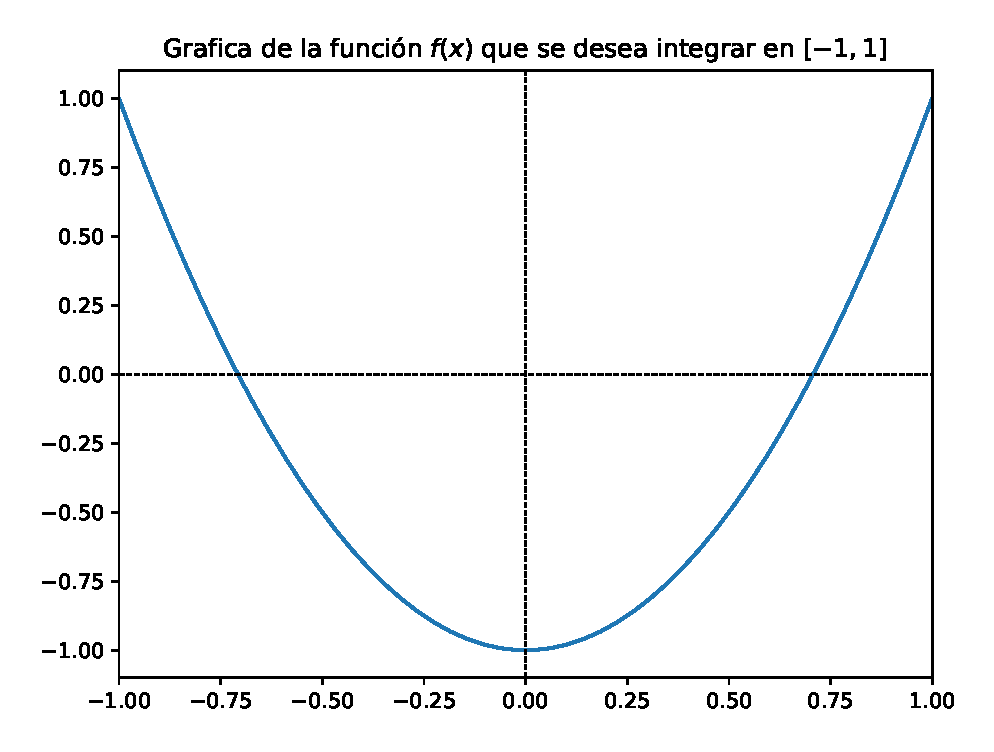
\includegraphics[scale=0.5]{Imagenes/integral_1_3_simpson.eps}
    \caption{Queremos calcular el valor del área debajo de la curva.}
\end{figure}
\end{frame}
\begin{frame}
\frametitle{Código para la solución}
Presentamos una propuesta para resolver el ejercicio, la función \funcionazul{qSimpson}, que integra la función \funcionazul{Func} en el intervalo $[a, b]$ usando la regla de Simpson con $n$ (impares) puntos de integración, requiere de los argumentos
\setbeamercolor{item projected}{bg=blue!70!black,fg=yellow}
\setbeamertemplate{enumerate items}[circle]
\begin{enumerate}[<+->]
\item La función $f(x)$
\item Los intervalos de integración $[x_{0}, x_{f}]$
\item El valor $n$ del número de intervalos.
\end{enumerate}
\end{frame}
\begin{frame}[allowframebreaks, fragile]
\begin{lstlisting}[caption=Código para el método de Simpson, style=FormattedNumber, basicstyle=\linespread{1.1}\ttfamily=\small, columns=fullflexible]
def qSimpson(Func, a, b, n):
    if (n % 2 == 0): n += 1
 
    h = (b-a)/(n-1)
    s_1_ = s_2_ = 0e0
    for i in range(2, n-2, 2): s_1_ += Func(a + i*h)
    for i in range(1, n-1, 2): s_2_ += Func(a + i*h)
 
    return (h/3)*(Func(a) + 4*s_2_ + 2*s_1_ + Func(b))

def f(x):
    return cos(2 * acos(x))

for i in range(1, 4):
    print ('Para n = {0:}'.format(i*2))
    print ('La integral vale {0:1.10f}'.format(qSimpson(f, -1., 1., i*2)))
\end{lstlisting}
\end{frame}
\begin{frame}[fragile]
\frametitle{Solución en la terminal}
\begin{verbatim}
Para n = 2
La integral vale = -0.6666666667

Para n = 4
La integral vale = -0.6666666667

Para n = 6
La integral vale = -0.6666666667
\end{verbatim}
\end{frame}
\begin{frame}
\frametitle{Sobre el código}
Hagamos algunos comentarios sobre el código anterior: Si el número recibido de puntos de integración $n$ es par, se corrige automáticamente al siguiente valor impar más alto, de modo que la fórmula de Simpson se puede aplicar a un número entero de tripletes de nodos, con las sumas de índice impar y de índice par calculado por separado.
\end{frame}
\begin{frame}
\frametitle{Sobre el código}
\setbeamercolor{item projected}{bg=blue!70!black,fg=yellow}
\setbeamertemplate{enumerate items}[circle]
\begin{enumerate}[<+->]
\item En la línea $2$ del código, se incrementa el valor de $n$, en caso de que sea par.
\item En la línea $6$, se tiene la suma en caso de que el índice sea impar.
\item En la línea $7$, se tiene la suma en caso de que el índice sea par.
\end{enumerate}
\end{frame}
\section{Métodos adaptativos de integración}
\frame{\tableofcontents[currentsection, hideothersubsections]}
\subsection*{Limitaciones de los métodos vistos}
\begin{frame}
\frametitle{Limitaciones de los métodos vistos}
Las implementaciones para el método del trapecio y la regla de Simpson presentadas anteriormente tienen un interés práctico pero limitado como tal: ya que, además de requerir el número de puntos de integración, no proporcionan una estimación de error para la integral.
\end{frame}
\begin{frame}
\frametitle{Nueva propuesta}
Una estrategia sencilla con una precisión de integración automática y control de avance en el dominio (malla) llamaría al \enquote{integrador} para los puntos obtenidos por sucesivas reducciones a la mitad y continuaría mientras la diferencia relativa entre aproximaciones consecutivas exceda una tolerancia admisible $\varepsilon$.
\end{frame}
\begin{frame}
\frametitle{Nueva propuesta}
Sin embargo, un inconveniente obvio sería la evaluación redundante del integrando en los nodos comunes de las mallas sucesivas.
\\
\bigskip
El cálculo de la integral con una precisión requerida por el \emph{método de reducción a la mitad} puede optimizarse significativamente al establecer una relación recursiva entre las aproximaciones consecutivas.
\end{frame}
\subsection{Método adaptativo del trapecio}
\begin{frame}
\frametitle{Método adaptativo del trapecio}
De acuerdo con la siguiente figura, se muestra las mallas de integración para las primeras cuatro etapas del proceso de reducción a la mitad.
\end{frame}
\begin{frame}
\frametitle{Método recursivo del trapecio}
\begin{figure}[h!]
    \centering
    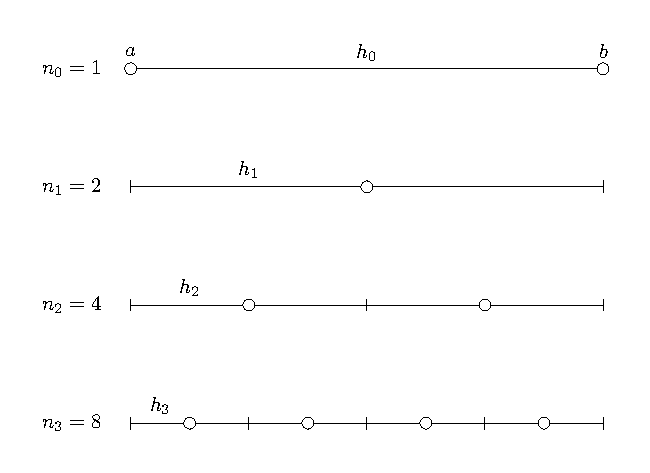
\includegraphics[scale=0.8]{Imagenes/integracion_08_recursiva.eps}
    % \caption{}
    % \label{}
\end{figure}
\end{frame}
\begin{frame}
\frametitle{Regla recursiva del trapecio}
La evaluación del integrando es necesaria únicamente en los nuevos puntos de integración (indicados por círculos) que dividen los subintervalos anteriores.
\\
\bigskip
Los valores de la función ya empleados se reutilizan implícitamente aplicando la relación de recurrencia entre dos aproximaciones consecutivas de la integral.
\end{frame}
\begin{frame}
\frametitle{Regla recursiva del trapecio}
Las primeras tres aproximaciones producidas por la regla trapezoidal son:
\begin{align*}
T_{0} &= h_{0} \, \left[ \dfrac{f(a)}{2} + \dfrac{f(b)}{2} \right], \hspace{0.5cm} h_{0} = b - a \\[0.5em]
\visible<2->{T_{1} &= h_{1} \, \left[ \dfrac{f(a)}{2} +  f(a + h_{1}) + \dfrac{f(b)}{2} \right], \hspace{0.5cm} h_{1} = \dfrac{h_{0}}{2}}\\[0.5em]
\end{align*}
\end{frame}
\begin{frame}
\frametitle{Regla recursiva del trapecio}
La tercera aproximación es:
\begin{align*}
T_{2} = h_{2} \, &\left[ \dfrac{f(a)}{2} +  f(a + h_{2}) + f(a + 2 \, h_{2}) + \right. \\  
&\left. + f(a + 3 \, h_{2}) + \dfrac{f(b)}{2} \right], \hspace{0.5cm} h_{2} = \dfrac{h_{1}}{2}
\end{align*}
\end{frame}
\begin{frame}
\frametitle{Regla de recurrencia}
La secuencia anterior se puede expresar en término de un proceso iterativo:
\begin{align*}
T_{0} &= \dfrac{h_{0}}{2} \, \left[ f(a) + f(b) \right], \hspace{0.5cm} h_{0} = b - a, \hspace{0.5cm} n_{0} = 1 \\[1em]
\visible<2->{T_{k} &= \dfrac{1}{2} \, \left[ T_{k-1} + h_{k-1} \, \sum_{i=1}^{n_{k-1}} f \left(a + \left( i - \dfrac{1}{2} \right) \, h_{k-1} \right) \right] \\[0.5em]
&h_{k} = \dfrac{h_{k-1}}{2}, \hspace{0.5cm} n_{k} = 2 \, n_{k-1}, \hspace{0.5cm} k = 1, 2, \ldots}
\end{align*}
\end{frame}
\begin{frame}
\frametitle{Regla de recurrencia}
donde $h_{k} = (b - a) / n_{k}$ es el espaciado de la malla después de la mitad del paso $k$, con $n_{k} = 2^{k}$ representando el número correspondiente de subintervalos o, equivalentemente, el número de nuevos puntos de integración relevantes para la próxima aproximación de la integral.
\end{frame}
\begin{frame}
\frametitle{Regla de recurrencia}
El proceso recursivo para $T_{0}$ y $T_{k}$ continua hasta que dos aproximaciones consecutivas de la integral se hacen indistinguibles para una precisión dada, es decir, la diferencia relativa
\begin{align*}
\dfrac{\abs{T_{k} - T_{k-1}}}{\abs{T_{k}}}
\end{align*}
considerado como el estimado del error relativo, éste es menor a una tolerancia establecida $\varepsilon$.
\end{frame}
\begin{frame}
\frametitle{Regla de recurrencia}
Para prevenir una singularidad en el cociente, cuando $T_{k} = 0$, el criterio de convergencia puede formularse convenientemente como
\begin{align*}
\abs{T_{k} - T_{k-1}} \leq \varepsilon \, \abs{T_{k}}
\end{align*}
\end{frame}
\subsection*{Código para el método adaptativo}
\begin{frame}
\frametitle{Código para el método adaptativo}
Se presenta un código que implementa el algoritmo adaptativo descrito basado en el método del trapecio.
\end{frame}
\begin{frame}
\frametitle{Código para el método adaptativo}
Para asegurarse que durante el proceso recursivo, el número de subintervalos $n$, elevado a la potencia de $2$, no exceda el valor máximo representable para un tipo de dato \emph{long} ($2^{31}$), el número máximo de iteraciones está limitado por \funcionazul{kmax} a un valor de 30.
\end{frame}
\begin{frame}
\frametitle{Código para el método adaptativo}
Sin embargo, si, debido a la débil convergencia, las iteraciones de \funcionazul{kmax} se agotan sin que la integración haya alcanzado la precisión solicitada \funcionazul{eps}, el ciclo de reducción a la mitad se deja con el contador \funcionazul{k} incrementado a \funcionazul{kmax + 1} y se muestra un mensaje de error.
\end{frame}
\begin{frame}[allowframebreaks, fragile]
\frametitle{Código para el método adaptativo}
\begin{lstlisting}[caption=Código para el método adaptativo del trapecio, style=FormattedNumber, basicstyle=\linespread{1.1}\ttfamily=\small, columns=fullflexible]
from math import fabs

def qAdaptTrapecio(Func, a, b, eps = 1e-6):
    kmax = 30
    h = b - a
    n = 1
    t_0_ = 0.5*h*(Func(a) + Func(b))

    for k in range(1, kmax+1):
        sumf = 0e0
        for i in range(1, n+1): sumf += Func(a + (i - 0.5)*h)
        t = 0.5*(t_0_ + h*sumf)
        if (k > 1):
            if (fabs(t-t_0_) <= eps*fabs(t)): break
            if (fabs(t) <= eps and fabs(t) <= fabs(t-t_0_)): break
        h *= 0.5; n *= 2
        t_0_ = t

    if (k >= kmax): print("Se excedio el numero de iteraciones en el metodo adaptativo !")

    return t
\end{lstlisting}
\end{frame}
\subsection{Método adaptativo de Simpson}
\begin{frame}
\frametitle{Método adaptativo de Simpson}
Sobre la base de la regla de Simpson, se puede idear un algoritmo adaptativo similar al del trapecio, aunque no independiente.
\end{frame}
\begin{frame}
\frametitle{Método adaptativo de Simpson}
De hecho, mientras que para la regla trapezoidal, se puede establecer una relación de recurrencia autoconsistente entre aproximaciones consecutivas obtenidas dividiendo el espaciado de malla (separación entre los puntos), para la regla de Simpson, no existe una relación algorítmica tan simple.
\end{frame}
\begin{frame}
\frametitle{Método adaptativo de Simpson}
En cambio, a partir de las primeras tres aproximaciones de la regla trapezoidal, las aproximaciones consecutivas a la fórmula de Simpson se pueden expresar en términos de la primera:
\begin{align*}
S_{1} &= \dfrac{h_{1}}{3} \bigg[ f(a) + 4 \, f(a + h_{1}) + f(b) \bigg] = \\
&= \dfrac{4 \, T_{1} - T_{0}}{3}
\end{align*}
\end{frame}
\begin{frame}
\frametitle{Método adaptativo de Simpson}
Para la segunda aproximación:
\begin{align*}
S_{2} &= \dfrac{h_{2}}{3} \bigg[ f(a) + 4 \, f(a + h_{2}) + 2 \, f(a + 2 \, h_{2}) + \\
&+ 4 \, f(a + 3 \, h_{2}) + f(b) \bigg] = \\
&= \dfrac{4 \, T_{2} - T_{1}}{3}
\end{align*}
\end{frame}
\begin{frame}
\frametitle{Regla generalizada}
Al generalizar, se obtiene la relación
\begin{align*}
S_{k} = \dfrac{4 \, T_{k} - T_{k-1}}{3}
\end{align*}
\end{frame}
\begin{frame}[fragile]
\frametitle{Regla generalizada}
Por lo tanto, se deduce que el algoritmo recursivo con control automático de pasos basado en la regla de Simpson puede describirse en términos de aproximaciones trapezoidales:
\end{frame}
\begin{frame}[fragile]
\frametitle{Regla generalizada}
\fontsize{12}{12}\selectfont
\begin{align*}
T_{0} &= \dfrac{h_{0}}{2} \, \left[ f(a) + f(b) \right], \hspace{0.5cm} h_{0} = b - a, \hspace{0.5cm} n_{0} = 1 \\[1em]
\visible<2->{T_{k} &= \dfrac{1}{2} \, \left[ T_{k-1} + h_{k-1} \, \sum_{i=1}^{n_{k-1}} f \left(a + \left( i - \dfrac{1}{2} \right) \, h_{k-1} \right) \right] \hspace{0.5cm} k = 1, 2, \ldots } \\[0.5em]
\visible<3->{S_{k} &= \dfrac{4 \, T_{k} - T_{k-1}}{3}, \hspace{0.5cm} h_{k} = \dfrac{h_{k-1}}{2}, \hspace{0.5cm} n_{k} = 2 \, n_{k-1}}
\end{align*}
\end{frame}
\begin{frame}
\frametitle{Criterio de convergencia}
El criterio de convergencia, implica que la diferencia relativa entre dos aproximaciones consecutivas de la fórmula de Simpson puede escribirse convenientemente como
\begin{align*}
\abs{S_{k} - S_{k-1}} \leq \varepsilon \, \abs{S_{k}}
\end{align*}
\end{frame}
\subsection*{Código para el método adaptativo}
\begin{frame}
\frametitle{Código para el método adaptativo}
Los argumentos, variables y constantes de la función \funcionazul{qAdaptSimpson}, que se presenta a continuación, mantienen la importancia que se les asignó en la función \funcionazul{qAdaptTrapecio}.
\end{frame}
\begin{frame}
\frametitle{Código para el método adaptativo}
A pesar de la conexión intrínseca con la regla trapezoidal, la tasa de convergencia del proceso se mejora debido a la aproximación superior proporcionada por la regla de Simpson ($\order{h^{4}}$) en comparación con $\order{h^{2}}$, que requiere, en general, significativamente menos iteraciones a la mitad para l misma precisión.
\end{frame}
\begin{frame}[allowframebreaks, fragile]
\frametitle{Código para el método adaptativo}
\begin{lstlisting}[caption=Código para el método adaptativo de Simpson, style=FormattedNumber, basicstyle=\linespread{1.1}\ttfamily=\small, columns=fullflexible]
from math import fabs

def qAdaptSimpson(Func, a, b, eps = 1e-6):
    kmax = 30

    h = b-a; n = 1
    s_0_ = t_0_ = 0.5*h*(Func(a) + Func(b))

    for k in range(1, kmax+1):
        sumf = 0e0
        for i in range(1, n+1): sumf += Func(a + (i-0.5)*h)
        t = 0.5*(t_0_ + h*sumf)
        s = (4*t - t_0_)/3
        if (k > 1):
            if (fabs(s - s_0_) <= eps*fabs(s)): break
            if (fabs(s) <= eps and fabs(s) <= fabs(s-s_0_)): break
        h *= 0.5; n *= 2
        s_0_ = s; t_0_ = t

    if (k >= kmax): print('Se excedieron el numero de iteraciones del metodo adaptativo de Simpson!')

    return s
\end{lstlisting}
\end{frame}
\section{Integración de Romberg}
\frame[allowframebreaks]{\tableofcontents[currentsection, hideothersubsections]}
\subsection{Definición de la integración de Romberg}
\begin{frame}
\frametitle{El método de integración de Romberg}
El método de Romberg puede considerarse como una generalización de las fórmulas de Newton-Cotes de orden superior del algoritmo adaptativo basado en la fórmula de Simpson que se desarrolló en la sección anterior.
\end{frame}
\begin{frame}
\frametitle{El método de integración de Romberg}
La reducción a la mitad del paso de integración está acompañada en el método de Romberg por el aumento recursivo adicional del orden del integrador elemental y esto produce una tasa de convergencia sin igual por cualquier otro esquema de cuadratura basado en las fórmulas de Newton-Cotes.
\end{frame}
\subsection*{Construcción del método}
\begin{frame}
\frametitle{Construcción del método}
En la sección anterior, establecimos la relación simple
\begin{align*}
S_{k} = \dfrac{4 \, T_{k} - T_{k-1}}{3}
\end{align*}
entre las aproximaciones $T_{k}$ de la regla trapezoidal para mallas de integración sucesivamente reducidas a la mitad y las aproximaciones correspondientes $S_{k}$ dadas por la fórmula de Simpson.
\end{frame}
\begin{frame}
\frametitle{Construcción del método}
Con el fin de generalizar este resultado a fórmulas de Newton-Cotes de orden superior, renombramos las aproximaciones trapezoidales como $R_{k,0}$:
\end{frame}
\begin{frame}
\frametitle{Construcción del método}
\begin{align*}
R_{0,0} &= h_{0} \left[ \dfrac{f(a)}{2} + \dfrac{f(b)}{2} \right], \hspace{0.5cm} h_{0} = b - a \\[0.5em]
\visible<2->{R_{1,0} &= h_{1} \left[ \dfrac{f(a)}{2} + f(a + h_{1}) + \dfrac{f(b)}{2} \right], \hspace{0.5cm} h_{1} = \dfrac{h_{0}}{2} \\[0.5em] }
\visible<3->{R_{2, 0} &= h_{2} \left[ \dfrac{f(a)}{2} + f(a + h_{2}) + f(a + 2 \, h_{2}) + \right. \\[0.5em]
&\left. + f(a + 3 \, h_{2}) + \dfrac{f(b)}{2} \right], \hspace{0.5cm} h_{2} = \dfrac{h_{1}}{2} }
\end{align*}
\end{frame}
\begin{frame}
\frametitle{Construcción del método}
El número de subintervalos para una aproximación dada $R_{k,0}$ y el espaciado de la malla correspondiente en la iteración $k$ están dados, respectivamente, por
\begin{align*}
n_{k} = 2^{k}, \hspace{1cm} h_{k} = \dfrac{(b-a)}{n_{k}}
\end{align*}
\end{frame}
\begin{frame}
\frametitle{Relación recursiva}
La relación recursiva que permite la evaluación óptima de $R_{k, 0}$, al reutilizar implícitamente los valores del integrando previamente calculados (evitando evaluaciones redundantes), es:
\end{frame}
\begin{frame}
\frametitle{Relación de recurrencia}
\begin{align*}
R_{k,0} &= \dfrac{1}{2} \left[ R_{k-1, 0} + h_{k-1} \sum_{i=1}^{n_{k-1}} f  \left(a + \left( i - \dfrac{1}{2} \right) \, h_{k-1} \right) \right], \\[0.5em]
&k = 1, 2,\ldots, k_{\max}
\end{align*}
que es la misma expresión para el método adaptativo del trapecio.
\end{frame}
\begin{frame}
\frametitle{Primeras aproximaciones}
Las dos primeras aproximaciones que se obtienen de la fórmula anterior son:
\begin{align*}
R_{1, 1} = \dfrac{h_{1}}{3} \bigg[ f(a) + 4 \, f(a + h_{1}) + f(b) \bigg] = \dfrac{4 \, R_{1, 0} - R_{0, 0}}{3}
\end{align*}
\end{frame}
\begin{frame}
\frametitle{Primeras aproximaciones}
La siguiente aproximación es:
\begin{align*}
R_{2, 1} &= \dfrac{h_{2}}{3} \bigg[ f(a) + 4 \, f(a + h_{2}) + 2 \, f(a + 2 \, h_{2}) + \\[0.5em]
&+ 4 \, f(a + 3\, h_{2}) +  f(b) \bigg] = \\[0.5em]
&= \dfrac{4 \, R_{2, 0} - R_{1, 0}}{3}
\end{align*}
\end{frame}
\begin{frame}
\frametitle{Relación general}
Entonces la relación general entre las aproximaciones basadas en la fórmula de Simpson y la regla del trapecio son de la forma:
\begin{align*}
R_{k, 1} &= \dfrac{4 \, R_{k, 0} - R_{k-1, 0}}{3} = \dfrac{4 \, R_{k, 0} - R_{k-1, 0}}{4 -1} \\[0.5em]
&k = 1, 2, \ldots, k_{\max}
\end{align*}
\end{frame}
\subsection*{Mejora en el esquema}
\begin{frame}
\frametitle{Mejora en el esquema}
Siguiendo con la idea de aumentar recursivamente el orden de la fórmula básica de Newton-Cotes, se espera que la primera aproximación del siguiente esquema de cuadratura se base en los nodos resultantes dividiendo los subintervalos característicos de la primera aproximación de la fórmula de Simpson, $R_{1,1}$ o de manera equivalente, en los nodos de la segunda aproximación, $R_{2,1}$.
\end{frame}
\begin{frame}
\frametitle{Mejora en el esquema}
Este requisito se cumple intrínsecamente mediante \emph{la fórmula de Boole de cinco puntos}, que esencialmente se aproxima al integrando por el polinomio de interpolación de Lagrange de cuarto orden:
\end{frame}
\subsection*{Fórmula de Boole}
\begin{frame}
\frametitle{Fórmula de Boole}
La fórmula de Boole es
\begin{align*}
\int_{x_{1}}^{x_{5}} f(x) \dd{x} &= \dfrac{2 \, h}{45} \bigg[ 7 \, f_{1} + 32 \, f_{2} + 12 \, f_{3} + \\[0.5em]
&+ 32 \, f_{4} + 7 \, f_{5} \bigg] - \dfrac{8 \, h^{7} \, f^{6} (\xi)}{945}
\end{align*}
\end{frame}
\begin{frame}
\frametitle{Aproximación con la fórmula de Boole}
La primera aproximación basada en la fórmula de Boole, se puede expresar en términos del paso de integración $h_{2}$, que corresponde a dos consecutivas iteraciones en donde se divide a la mitad el intervalo completo $[a, b]$
\end{frame}
\begin{frame}
\frametitle{Aproximación con la fórmula de Boole}
La aproximación queda como
\begin{align*}
R_{2, 2} &= \dfrac{2 \, h}{45} \bigg[ 7 \, f{a} + 32 \, f(a + h_{2}) + 12 \, f(a + 2 \, h_{2}) + \\[0.5em]
&+ 32 \, f(a + 3 \, h_{2}) + 7 \, f(b) \bigg] 
\end{align*}
\end{frame}
\begin{frame}
\frametitle{Aproximación con la fórmula de Boole}
Además, puede estar relacionado con las dos primeras aproximaciones proporcionadas por la fórmula de Simpson:
\begin{align*}
R_{2, 2} = \dfrac{16 \, R_{2, 1} - R_{1, 1}}{15} = \dfrac{4^{2} \, R_{2, 1}- R_{1, 1}}{4^{2} - 1}
\end{align*}
\end{frame}
\subsection*{Consecuencias del esquema}
\begin{frame}
\frametitle{Consecuencias del esquema}
Se puede anticipar fácilmente que el aumento del orden del esquema de cuadratura básica implica duplicar el número de subintervalos característicos de $2^{k}$ ($2$ para la fórmula de Simpson) a $2^{k + 1}$ ($4$ para la fórmula de Boole) e, inherentemente, duplicar el orden de Polinomio de interpolación de Lagrange por el cual se aproxima el integrando.
\end{frame}
\begin{frame}
\frametitle{Consecuencias del esquema}
En consecuencia, a excepción de la aproximación inicial $R_{0, 0}$, todas las aproximaciones superiores se basan en mallas de integración con números impares de nodos ($2^{k} + 1$).
\end{frame}
\subsection*{Relación de recurrencia}
\begin{frame}
\frametitle{Relación de recurrencia}
Se puede demostrar en general, aunque no sin cierta dificultad, que la relación de recurrencia entre la aproximación $R_{k, j}$ (resultante de la aplicación de la fórmula de Newton-Cotes de subintervalos de orden $2^{j}$ a $2^{k}$) y las aproximaciones $R_{k, j-1}$ y $R_{k-1, j-1}$ basado en la cuadratura inferior del orden $2^{j-1}$ es:
\end{frame}
\begin{frame}
\frametitle{Relación de recurrencia}
Relación de recurrencia para $R_{k, j}$:
\begin{align*}
R_{k, j} &= \dfrac{4^{j} \, R_{k, j-1} - R_{k-1, j-1}}{4^{j}-1} \\[0.5em]
&j = 1, 2, \ldots, k, \hspace{0.5cm} k = 1, 2, \ldots,  k_{\max}
\end{align*}
\end{frame}
\subsection*{Máxima aproximación}
\begin{frame}
\frametitle{Máximo de intervalos}
Para un número dado de subintervalos $(2^{k})$, el orden de las fórmulas de Newton-Cotes aplicables $(2^{j})$ obviamente no puede exceder el número de subintervalos y, por tanto, $j \leq k$.
\end{frame}
\subsection*{Aproximación más baja}
\begin{frame}
\frametitle{Aproximación más baja}
Por el contrario, la aproximación más baja del esquema de orden $2^{j}$ debe ser $R_{j, j}$.
\\
\bigskip
Por lo tanto, es natural organizar todas las aproximaciones $R_{k, j}$ de la integral en un arreglo triangular con "predecesores" y "descendientes":
\end{frame}
\subsection*{Arreglo triangular}
\begin{frame}
\frametitle{Arreglo triangular}
\begin{table}
\centering
\begin{tabular}{c | c c c c c}
$n_{k}$ & Trapecio & Simpson & Boole & &  \\ \hline
$1$ & $R_{0, 0}$ & & & & \\
$2$ & $R_{1, 0}$ & $R_{1, 1}$ & & & \\
$2^{2}$ & $R_{2, 0}$ & $R_{2, 1}$ & $R_{2, 2}$& & \\
$\vdots$ & $\vdots$ & $\vdots$ &  & $\ddots$ & \\
$2^{k_{\max}}$ & $R_{k_{\max}, 0}$ & $R_{k_{\max}, 1}$ & \ldots & \ldots & $R_{k_{\max}, k_{\max}}$     
\end{tabular}
\end{table}
\end{frame}
\begin{frame}
\frametitle{Arreglo triangular}
La columna $j$ contiene las aproximaciones basadas en la fórmula de Newton-Cotes de orden $2^{j}$ para números sucesivamente duplicados de subintervalos (tamaños de subintervalos reducidos a la mitad).
\end{frame}
\subsection*{El mejor valor de la integral}
\begin{frame}
\frametitle{El mejor valor de la integral}
La evaluación óptima de la integral se puede lograr completando el arreglo triangular anterior de forma recursiva de arriba hacia abajo, determinando para cada fila $k$ las aproximaciones basadas en todas las fórmulas de Newton-Cotes aplicables en la malla respectiva de $2^{k}$ puntos de integración (comenzando con la regla trapezoidal y terminando con el esquema de orden $2^{k}$).
\end{frame}
\begin{frame}
\frametitle{El mejor valor de la integral}
Específicamente, los elementos de la matriz se evalúan en el orden $R_{0, 0}, (R_{1, 0}, R_{1, 1}), (R_{2, 0}, R_{2, 1}, R_{2, 2})$.
\\
\bigskip
Dentro de un número dado de iteraciones de reducción a la mitad, $k_{\max}$, que, sin embargo, no necesita ser arreglado de antemano, la mejor aproximación de la integral la proporciona el descendiente diagonal en el última fila completada: $R_{k_{\max}, k_{\max}}$.
\end{frame}
\begin{frame}
\frametitle{El mejor valor de la integral}
La esencia del método de Romberg consiste, por lo tanto, en completar recursivamente el conjunto de aproximaciones $R_{k, j}$ de la integral, que se presenta de la forma:
\end{frame}
\begin{frame}
\frametitle{El mejor valor de la integral}
\begin{align}
R_{0, 0} &= \dfrac{h_{0}}{2} \bigg[ f(a) +  f(b) \bigg] \hspace{0.5cm} h_{0} = b - a, \hspace{0.5cm} n_{0} = 1 \label{eq:ecuacion_10_47} \\[0.5em]
R_{k, 0} &= \dfrac{1}{2} \left[ R_{k-1, 0} + h_{k-1} \sum_{i=1}^{n_{k-1}} f \left( a + \left( i - \dfrac{1}{2} \right) \, h_{k-1} \right) \right] \label{eq:ecuacion_10_48} \\[0.5em]
R_{k, j} &= \dfrac{4^{j} \, r_{k, j-1} - R_{k-1, j-1}}{4^j - 1} \hspace{0.5cm} j = 1, 2, \ldots, k \label{eq:ecuacion_10_49} \\[0.5em]
&h_{k} = \dfrac{h_{k-1}}{2} \hspace{0.5cm} n_{k} = 2 \, n_{k-1}, \hspace{0.5cm} k = 1, 2, \ldots, k_{\max} \nonumber
\end{align}
\end{frame}
\begin{frame}
\frametitle{Manejo del arreglo triangular}
El elemento inicial $R_{k, 0}$ de cada nueva fila $k$ se calcula de acuerdo con la ec. (\ref{eq:ecuacion_10_48}) dividiendo a la mitad la malla de integración y utilizando su predecesor \enquote{trapezoidal} $R_{k-1, 0}$.
\end{frame}
\begin{frame}
\frametitle{Manejo del arreglo triangular}
Continuando a lo largo de una fila con un nuevo $R_{k, j}$ se lleva a cabo de acuerdo con la ec. (\ref{eq:ecuacion_10_47}) utilizando las estimaciones $R_{k, j-1}$ y $R_{k-1, j-1}$ dadas por la fórmula anterior de Newton-Cotes.
\end{frame}
\subsection*{Tolerancia de ejecución}
\begin{frame}
\frametitle{Tolerancia de ejecución}
El proceso iterativo debe continuarse hasta que la diferencia relativa entre dos aproximaciones diagonales consecutivas sea menor que una tolerancia predefinida $\varepsilon$:
\begin{align*}
\abs{R_{k, k} - R_{k-1, k-1}} \leq \varepsilon \, \abs{R_{k, k}}
\end{align*}
\end{frame}
\begin{frame}
\frametitle{Comentario sobre el esquema}
Una estrategia alternativa sería llenar el arreglo triangular anterior, en forma de columna de izquierda a derecha.
\\
\bigskip
Sin embargo, esto requeriría fijar el número máximo de iteraciones de reducción a la mitad $k_{\max}$ por adelantado y evaluar todas las aproximaciones en cada columna hasta que se cumpla la convergencia para una estimación diagonal $R_{k, k}$
\end{frame}
\begin{frame}
\frametitle{Comentario sobre el esquema}
En este punto, si $k < k_{\max}$, las estimaciones ya calculadas ubicadas debajo de la fila $k$ serían innecesarias, haciendo que el algoritmo sea ineficiente.
\end{frame}
\subsection{Código para el método de Romberg}
\begin{frame}
\frametitle{Código para el método de Romberg}
Se presenta un código para el método de Romberg en la función \funcionazul{qRomberg}, que tiene los mismos parámetros que las funciones \funcionazul{qAdaptTrapz} y \funcionazul{qAdaptSimpson}.
\end{frame}
\begin{frame}
\frametitle{Código para el método de Romberg}
En lugar del arreglo triangular de aproximaciones $R_{k, j}$, la implementación usa sólo dos arreglos unidimensionales para las dos filas consecutivas más recientes, \funcionazul{r1} y \funcionazul{r2}, que se desplazan al final de cada iteración de subintervalo de reducción a la mitad.
\end{frame}
\begin{frame}
\frametitle{Código para el método de Romberg}
Al igual que en el caso de las funciones \funcionazul{qAdaptTrapz} y \funcionazul{qAdaptSimpson}, el número de iteraciones a la mitad está limitado a $30$, lo que corresponde a un máximo de $230$ puntos de integración (la mayor potencia de 2 representable por una variable de tipo largo).
\end{frame}
\begin{frame}
\frametitle{Código para el método de Romberg}
Cada iteración a la mitad del espacio de integración comienza con la evaluación de la integral basada en la fórmula trapezoidal.
\\
\bigskip
El orden de la cuadratura básica se eleva de forma recursiva y se verifica la convergencia del proceso.
\end{frame}
\begin{frame}
\frametitle{Código para el método de Romberg}
Si no se logra la precisión \funcionazul{eps} solicitada después de recorrer todas las fórmulas de Newton Cotes aplicables para el número actual de puntos de malla, el siguiente paso de reducción a la mitad se prepara duplicando el número de subintervalos (reduciendo a la mitad el espacio de malla).
\end{frame}
\begin{frame}
\frametitle{Código para el método de Romberg}
Si no se logra la convergencia dentro de las iteraciones de reducción a la mitad permitidas por \funcionazul{kmax}, se emite un mensaje de advertencia.
\end{frame}
\begin{frame}[allowframebreaks, fragile]
\frametitle{Código en \texttt{pyhton}}
\begin{lstlisting}[caption=Código para el método de Romberg, style=FormattedNumber, basicstyle=\linespread{1.1}\ttfamily=\small, columns=fullflexible]
from math import fabs

def qRomberg(Func, a, b, eps = 1e-6):

    kmax = 30
    r_1_ = [0]*(kmax + 1)
    r_2_ = [0]*(kmax + 1)

    h = b - a; n = 1

    r_1_[0] = 0.5*h*(Func(a) + Func(b))
    
    for k in range(1, kmax+1):
        sumf = 0e0
        for i in range(1, n+1): sumf += Func(a+(i-0.5)*h)
        r_2_[0] = 0.5*(r_1_[0] + h*sumf)
        f = 1e0
        for j in range(1, k+1):
            f *= 4
            r_2_[j] = (f*r_2_[j-1] - r_1_[j-1])/(f-1)

        if (k > 1):
            if (fabs(r_2_[k] - r_1_[k-1]) <= eps*fabs(r_2_[k])): break
            if (fabs(r_2_[k]) <= eps and fabs(r_2_[k]) <= fabs(r_2_[k] - r_1_[k-1])): break
        h *= 0.5; n *= 2
        for j in range(0, k+1): r_1_[j] = r_2_[j]

    if (k >= kmax):
        print("Metodo de Romberg: Se excedieron las iteraciones!")
        k -= 1

    return r_2_[k]
\end{lstlisting}
\end{frame}
\begin{frame}
\frametitle{Ejercicio}
Para revisar la eficiencia de los métodos adapativos de integración, considera la siguiente integral:
\begin{align*}
\int_{0}^{1} x^{3} \, \exp(-x) \dd{x} &=  6 - 16 \, \exp(-1) \\
&=  0.11392894125692\ldots
\end{align*}
\pause
Calcula el valor de la integral usando los métodos adaptativos del Trapecio, de Simpson y de Romberg, con una precisión de $\varepsilon = \num{d-14}$.
\end{frame}
\begin{frame}
\frametitle{Completa la tabla}
Como ejercicio a cuenta, completa la siguiente tabla (nota: tendrás que hacer un pequeño ajuste en tu código para incluir la información requerida)
\begin{table}
\centering
\begin{tabular}{l c c c}
Método & Integral & Error & No. iteraciones \\\hline
Adapt. Trapecio & & & \\\hline
Adapt. Simpson & & & \\\hline
Romberg & & & \\\hline
\end{tabular}
\end{table}
\end{frame}
% \begin{frame}
% \frametitle{Integración de Romberg}
% La integración de Romberg combina la regla del trapecio con la extrapolación de Richardson. 
% \\
% \bigskip
% Usemos la siguiente notación:
% \begin{align*}
% R_{i, 1} = I_{i}
% \end{align*}
% donde $I_{i}$ representa el valor aproximado de $\int_{a}^{b} \: f(x) \dd{x}$ calculado con el método recursivo del trapecio, usando $2^{i - 1}$ bloques.
% \end{frame}
% \begin{frame}
% \frametitle{Integración de Romberg}
% Recordemos que el error en esta aproximación es $E = c_{1} \: h^{2} + c_{2} \: h^{4} + \ldots$ donde
% \begin{align*}
% h = \dfrac{b - a}{2^{i - 1}}
% \end{align*}
% es el ancho del bloque.
% \end{frame}
% \subsection*{Inicio de la integración}
% \begin{frame}
% \frametitle{Inicio de la integración}
% La integración de Romberg inicia con el cálculo de $R_{1, 1} = I_{1}$ (un bloque) y $R_{2, 1} = I_{2}$ (dos bloques) a partir de la regla del trapecio.
% \end{frame}
% \begin{frame}
% \frametitle{Cancelación término dominante}
% El término dominante $c_{1} \: h^{2}$ es entonces eliminado por la extrapolación de Richardson.
% \\
% \bigskip
% Usando $p = 2$ (el exponente en el término dominante) e indicando el resultado por $R_{2, 2}$, tenemos que:
% \begin{align*}
% R_{2, 2} = \dfrac{2^{2} \: R_{2, 1} - R_{1, 1}}{2^{2} - 1} = \dfrac{4}{3} \: R_{2, 1} - \dfrac{1}{3} \: R_{1, 1}
% \end{align*}
% \end{frame}
% \begin{frame}
% \frametitle{Notación para los cálculos}
% Es conveniente guardar los resultados en un arreglo con la siguiente forma:
% \begin{align*}
% \begin{bmatrix}
% R_{1, 1} & \\
% R_{2, 1} & R_{2, 2}
% \end{bmatrix}
% \end{align*}
% \end{frame}
% \begin{frame}
% \frametitle{Aumentando los bloques}
% El siguiente paso es calcular $R_{3, 1} = I_{3}$ (cuatro bloques) y repetir la extrapolación de Richardson con $R_{2, 1}$ y $R_{3, 1}$, guardando los resultados como $R_{3, 2}$:
% \begin{align*}
% R_{3, 2} = \dfrac{4}{3} \: R_{3,1} - \dfrac{1}{3} \: R_{2,1}
% \end{align*}
% \end{frame}
% \begin{frame}
% \frametitle{Elementos obtenidos}
% Los elementos del arreglo $R$ calculados hasta el momento son:
% \begin{align*}
% \begin{bmatrix}
% R_{1, 1} & \\
% R_{2, 1} & R_{2, 2} \\
% R_{3, 1} & R_{3, 2}
% \end{bmatrix}
% \end{align*}
% Los elementos de la segunda columna tienen un error del orden $c_{2} \: h^{4}$, el cual puede ser eliminado con la extrapolación de Richardson.
% \end{frame}
% \begin{frame}
% \frametitle{Usando un valor para \texttt{p}}
% Usando $p = 4$, obtenemos:
% \begin{align*}
% R_{3, 3} = \dfrac{2^{4} \: R_{3, 2}-R_{2, 2}}{2^{4} - 1} = \dfrac{16}{15} \: R_{3, 2} - \dfrac{1}{15} \: R_{2, 2}
% \end{align*}
% El resultado tiene ahora un error del orden $\order{h^{6}}$.
% \end{frame}
% \begin{frame}
% \frametitle{Usando un valor para \texttt{p}}
% El arreglo se ha expandido ahora como
% \begin{align*}
% \begin{bmatrix}
% R_{1, 1} &  & \\
% R_{2, 1} & R_{2, 2} & \\
% R_{3, 1} & R_{3, 2} & R_{3, 3}
% \end{bmatrix}
% \end{align*}
% \end{frame}
% \begin{frame}
% \frametitle{Resultados de otro cálculo}
% Luego de otra ronda de cálculos, se tiene
% \begin{align*}
% \begin{bmatrix}
% R_{1, 1} &  & & \\
% R_{2, 1} & R_{2, 2} & & \\
% R_{3, 1} & R_{3, 2} & R_{3, 3} & \\
% R_{4, 1} & R_{4, 2} & R_{4, 3} & R_{4, 4}
% \end{bmatrix}
% \end{align*}
% donde el error en $R_{4, 4}$ es del orden de $\order{h^{8}}$.
% \\
% \bigskip
% \pause
% \textoazul{Nótese que la estimación con mayor precisión es siempre el último término de la diagonal}.
% \end{frame}
% \begin{frame}
% \frametitle{Punto de paro}
% Este proceso continua hasta que la diferencia entre dos términos sucesivos de la diagonal son lo suficientemente pequeños.
% \end{frame}
% \subsection*{Fórmula general}
% \begin{frame}
% \frametitle{Fórmula general}
% La fórmula general para la extrapolación es:
% \begin{align*}
% R_{i, j} = \dfrac{4^{j - 1} \: R_{i, j - 1} - R_{i - 1, j - 1} }{4^{j - 1} - 1} \hspace{1cm} i > 1, \hspace{0.3cm} j = 2, 3, \ldots, i
% \end{align*}
% \end{frame}
% \begin{frame}[fragile]
% \frametitle{El proceso de integración}
% Esquemáticamente lo que tenemos es:
% \begin{figure}
%   \centering
%   \includestandalone{Figuras/integracion_07}
% \end{figure}
% \end{frame}
% \begin{frame}
% \frametitle{Multiplicadores}
% Donde los multiplicadores $\alpha$ y $\beta$ dependen de $j$ de la siguiente manera:
% \fontsize{12}{12}\selectfont
% \begin{center}
% \begin{tabular}{c | c | c | c | c | c}
% \hline
% j & $2$ & $3$ & $4$ & $5$ & $6$ \\ \hline
% $\alpha$ & $-1/3$ & $-1/15$ & $-1/63$ & $-1/255$ & $-1/1023$ \\ \hline
% $\beta$ & $4/3$ & $16/15$ & $64/63$ & $256/255$ & $1024/1023$ \\ \hline
% \end{tabular}
% \end{center}
% \end{frame}
% \begin{frame}
% \frametitle{Manejo triangular}
% El arreglo triangular es conveniente para manipularlo computacionalmente hablando.
% \\
% \bigskip
% La aplicación del algoritmo de Romberg puede llevarse dentro de una matriz de una dimensión.
% \end{frame}
% \begin{frame}
% \frametitle{Aprovechando las expresiones}
% Luego de la primera extrapolación, $R_{1,1}$ ya no se ocupa de nuevo, por lo que podemos re-emplazarla con $R_{2,2}$, por tanto, tenemos en el arreglo
% \begin{align*}
% \begin{bmatrix}
% R^{\prime}_{1} = R_{2, 2} \\
% R^{\prime}_{2} = R_{2, 1}
% \end{bmatrix}
% \end{align*}
% \end{frame}
% \begin{frame}
% \frametitle{Aprovechando las expresiones}
% En la segunda extrapolación, $R_{3, 2} $ sobre-escribe a $R_{2, 1}$ y $R_{3, 3}$ re-emplaza a $R_{2, 2}$, entonces el arreglo queda
% \begin{align*}
% \begin{bmatrix}
% R^{\prime}_{1} = R_{3, 3} \\
% R^{\prime}_{2} = R_{3, 2} \\
% R^{\prime}_{3} = R_{3, 1}
% \end{bmatrix}
% \end{align*} 
% \pause
% Y así podemos continuar. $R^{\prime}_{1}$ contiene siempre el mejor resultado.
% \end{frame}
% \subsection*{Expresión general para la extrapolación}
% \begin{frame}
% \frametitle{Expresión general para la extrapolación}
% La fórmula de extrapolación para el k-ésima vuelta, es:
% \begin{align*}
% R^{\prime}_{j} = \dfrac{4^{k - j} \: R^{\prime}_{j + 1} - R^{\prime}_{j}}{4^{k - j} - 1}, \hspace{0.8cm} j = k - 1, k - 2, \ldots, 1
% \end{align*}
% \end{frame}
% \begin{frame}
% \frametitle{Ejemplo}
% Usando la integración de Romberg, evalúa
% \[ \int_{0}^{\pi} \: f(x) \dd{x}\]
% donde $f(x) = \sin(x)$
% \end{frame}
% \begin{frame}
% \frametitle{Primera parte: Regla del trapecio recursiva}
% \begin{align*}
% R_{1, 1} &= I(\pi) = \frac{\pi}{2} \bigg[ f(0) + f(\pi) \bigg] = 0 \\[0.5em]
% \visible<2->{R_{2, 1} &= I \left(\frac{\pi}{2}\right) = \frac{1}{2} \: I(\pi) +  \frac{\pi}{2} \: f \left(\frac{\pi}{2} \right) = 1.5708} \\[0.5em]
% \visible<3->{R_{3, 1} &= I \left(\frac{\pi}{4} \right) = \frac{1}{2} \: I \left(\frac{\pi}{2} \right) + \frac{\pi}{4} \left[ f \left(\frac{\pi}{4} \right) + f \left(\frac{3 \: \pi}{4} \right) \right] = \\[0.5em]
% &= 1.8961}
% \end{align*}
% \end{frame}
% \begin{frame}
% \frametitle{Primera parte: Regla del trapecio recursiva}
% \begin{align*}
% R_{4, 1} &= I \left( \frac{\pi}{8} \right) = \frac{1}{2} \: I \left( \frac{\pi}{4} \right) + \frac{\pi}{8} \left[ f \left( \frac{\pi}{8} \right) + f \left( \frac{3 \: \pi}{8} \right) + \right. \\[0.5em]
% & \left. + f \left( \frac{5 \: \pi}{8} \right) + f \left( \frac{7 \: \pi}{8} \right) \right] = \\[0.5em]
% &= 1.9742
% \end{align*}
% \end{frame}
% \begin{frame}
% \frametitle{Segunda parte: Extrapolación de Richardson}
% Usando las fórmulas de extrapolación, construimos la siguiente tabla:
% \fontsize{12}{12}\selectfont
% \begin{align*}
% \begin{bmatrix}
% R_{1, 1} &         &         & \\
% R_{2, 1} & R_{2, 2} &         & \\
% R_{3, 1} & R_{3, 2} & R_{3, 3} & \\
% R_{4, 1} & R_{4, 2} & R_{4, 3} & R_{4, 4} 
% \end{bmatrix}
% =
% \begin{bmatrix}
% 0      &        &        & \\
% 1.5708 & 2.0944 &        & \\
% 1.8961 & 2.0046 & 1.9986 & \\
% 1.9742 & 2.0003 & 2.0000 & 2.0000
% \end{bmatrix}
% \end{align*}
% \end{frame}
% \begin{frame}
% \frametitle{Segunda parte: Extrapolación de Richardson}
% De acuerdo al procedimiento, vemos que converge, por tanto
% \begin{align*}
% \int_{0}^{\pi} \: \sin(x) \dd{x} = R_{4, 4} = 2.0000
% \end{align*}
% que es el resultado exacto.
% \end{frame}
% \subsection{Código para el método de Romberg}
% \begin{frame}
% \frametitle{Propuesta de código}
% El algoritmo para la integración de Romberg se implementa en la función \funcionazul{romberg}.
% \\
% \bigskip
% Devuelve la integral $I$ y el número de paneles utilizados $n$. La extrapolación de Richardson la lleva a cabo la subfunción \funcionazul{richardson}.
% \end{frame}
% \begin{frame}[allowframebreaks, fragile]
% \frametitle{Código para el método de Romberg}
% \begin{lstlisting}[caption=Código para la función trapecios, style=FormattedNumber, basicstyle=\linespread{1.1}\ttfamily=\small, columns=fullflexible]
% def Romberg(f, x_0_, xf, eps=1.0e-6):
% n = 1
% i = 1
% R = [[trapecios(f, x_0_, xf, n)]]
% while True:
%     n *= 2
%     i += 1
%     R += [[trapecios(f,x0,xf,n)]]
%     j = 0
%     for k in range(i-1,0,-1):
%         j += 1
%         R[k-1] += [R[k][j-1]+1./(4**j-1)*(R[k][j-1]-R[k-1][j-1])]
%     if abs(R[0][j]-R[1][j-1]) < Eps:
%         return R[0][j], n
 
% \end{lstlisting}
% \end{frame}
\end{document}